\documentclass[twoside]{book}

% Packages required by doxygen
\usepackage{fixltx2e}
\usepackage{calc}
\usepackage{doxygen}
\usepackage[export]{adjustbox} % also loads graphicx
\usepackage{graphicx}
\usepackage[utf8]{inputenc}
\usepackage{makeidx}
\usepackage{multicol}
\usepackage{multirow}
\PassOptionsToPackage{warn}{textcomp}
\usepackage{textcomp}
\usepackage[nointegrals]{wasysym}
\usepackage[table]{xcolor}

% NLS support packages
\usepackage[brazil]{babel}
% Font selection
\usepackage[T1]{fontenc}
\usepackage[scaled=.90]{helvet}
\usepackage{courier}
\usepackage{amssymb}
\usepackage{sectsty}
\renewcommand{\familydefault}{\sfdefault}
\allsectionsfont{%
  \fontseries{bc}\selectfont%
  \color{darkgray}%
}
\renewcommand{\DoxyLabelFont}{%
  \fontseries{bc}\selectfont%
  \color{darkgray}%
}
\newcommand{\+}{\discretionary{\mbox{\scriptsize$\hookleftarrow$}}{}{}}

% Page & text layout
\usepackage{geometry}
\geometry{%
  a4paper,%
  top=2.5cm,%
  bottom=2.5cm,%
  left=2.5cm,%
  right=2.5cm%
}
\tolerance=750
\hfuzz=15pt
\hbadness=750
\setlength{\emergencystretch}{15pt}
\setlength{\parindent}{0cm}
\setlength{\parskip}{3ex plus 2ex minus 2ex}
\makeatletter
\renewcommand{\paragraph}{%
  \@startsection{paragraph}{4}{0ex}{-1.0ex}{1.0ex}{%
    \normalfont\normalsize\bfseries\SS@parafont%
  }%
}
\renewcommand{\subparagraph}{%
  \@startsection{subparagraph}{5}{0ex}{-1.0ex}{1.0ex}{%
    \normalfont\normalsize\bfseries\SS@subparafont%
  }%
}
\makeatother

% Headers & footers
\usepackage{fancyhdr}
\pagestyle{fancyplain}
\fancyhead[LE]{\fancyplain{}{\bfseries\thepage}}
\fancyhead[CE]{\fancyplain{}{}}
\fancyhead[RE]{\fancyplain{}{\bfseries\leftmark}}
\fancyhead[LO]{\fancyplain{}{\bfseries\rightmark}}
\fancyhead[CO]{\fancyplain{}{}}
\fancyhead[RO]{\fancyplain{}{\bfseries\thepage}}
\fancyfoot[LE]{\fancyplain{}{}}
\fancyfoot[CE]{\fancyplain{}{}}
\fancyfoot[RE]{\fancyplain{}{\bfseries\scriptsize Gerado por Doxygen }}
\fancyfoot[LO]{\fancyplain{}{\bfseries\scriptsize Gerado por Doxygen }}
\fancyfoot[CO]{\fancyplain{}{}}
\fancyfoot[RO]{\fancyplain{}{}}
\renewcommand{\footrulewidth}{0.4pt}
\renewcommand{\chaptermark}[1]{%
  \markboth{#1}{}%
}
\renewcommand{\sectionmark}[1]{%
  \markright{\thesection\ #1}%
}

% Indices & bibliography
\usepackage{natbib}
\usepackage[titles]{tocloft}
\setcounter{tocdepth}{3}
\setcounter{secnumdepth}{5}
\makeindex

% Hyperlinks (required, but should be loaded last)
\usepackage{ifpdf}
\ifpdf
  \usepackage[pdftex,pagebackref=true]{hyperref}
\else
  \usepackage[ps2pdf,pagebackref=true]{hyperref}
\fi
\hypersetup{%
  colorlinks=true,%
  linkcolor=blue,%
  citecolor=blue,%
  unicode%
}

% Custom commands
\newcommand{\clearemptydoublepage}{%
  \newpage{\pagestyle{empty}\cleardoublepage}%
}

\usepackage{caption}
\captionsetup{labelsep=space,justification=centering,font={bf},singlelinecheck=off,skip=4pt,position=top}

%===== C O N T E N T S =====

\begin{document}

% Titlepage & ToC
\hypersetup{pageanchor=false,
             bookmarksnumbered=true,
             pdfencoding=unicode
            }
\pagenumbering{alph}
\begin{titlepage}
\vspace*{7cm}
\begin{center}%
{\Large Servidor \\[1ex]\large 1.\+0 }\\
\vspace*{1cm}
{\large Gerado por Doxygen 1.8.14}\\
\end{center}
\end{titlepage}
\clearemptydoublepage
\pagenumbering{roman}
\tableofcontents
\clearemptydoublepage
\pagenumbering{arabic}
\hypersetup{pageanchor=true}

%--- Begin generated contents ---
\chapter{$<$em$>$Namespaces$<$/em$>$}
\section{Lista de Namespaces}
Esta é a lista de todos os Namespaces com suas respectivas descrições\+:\begin{DoxyCompactList}
\item\contentsline{section}{\mbox{\hyperlink{namespace_ui}{Ui}} }{\pageref{namespace_ui}}{}
\end{DoxyCompactList}

\chapter{Índice Hierárquico}
\section{Hierarquia de Classes}
Esta lista de hierarquias está parcialmente ordenada (ordem alfabética)\+:\begin{DoxyCompactList}
\item Q\+Main\+Window\begin{DoxyCompactList}
\item \contentsline{section}{Main\+Window}{\pageref{class_main_window}}{}
\end{DoxyCompactList}
\end{DoxyCompactList}

\chapter{Índice dos Componentes}
\section{Class List}
Here are the classes, structs, unions and interfaces with brief descriptions\+:\begin{DoxyCompactList}
\item\contentsline{section}{\mbox{\hyperlink{class_main_window}{Main\+Window}} }{\pageref{class_main_window}}{}
\item\contentsline{section}{\mbox{\hyperlink{class_plotter}{Plotter}} }{\pageref{class_plotter}}{}
\end{DoxyCompactList}

\chapter{Índice dos Arquivos}
\section{File List}
Here is a list of all files with brief descriptions\+:\begin{DoxyCompactList}
\item\contentsline{section}{C\+:/\+Users/mateu/\+Documents/\+Cliente\+\_\+\+Consumidor/\mbox{\hyperlink{main_8cpp}{main.\+cpp}} }{\pageref{main_8cpp}}{}
\item\contentsline{section}{C\+:/\+Users/mateu/\+Documents/\+Cliente\+\_\+\+Consumidor/\mbox{\hyperlink{mainwindow_8cpp}{mainwindow.\+cpp}} }{\pageref{mainwindow_8cpp}}{}
\item\contentsline{section}{C\+:/\+Users/mateu/\+Documents/\+Cliente\+\_\+\+Consumidor/\mbox{\hyperlink{mainwindow_8h}{mainwindow.\+h}} }{\pageref{mainwindow_8h}}{}
\item\contentsline{section}{C\+:/\+Users/mateu/\+Documents/\+Cliente\+\_\+\+Consumidor/\mbox{\hyperlink{plotter_8cpp}{plotter.\+cpp}} }{\pageref{plotter_8cpp}}{}
\item\contentsline{section}{C\+:/\+Users/mateu/\+Documents/\+Cliente\+\_\+\+Consumidor/\mbox{\hyperlink{plotter_8h}{plotter.\+h}} }{\pageref{plotter_8h}}{}
\end{DoxyCompactList}

\chapter{$<$em$>$Namespace$<$/em$>$}
\hypertarget{namespace_ui}{}\section{Ui Namespace Reference}
\label{namespace_ui}\index{Ui@{Ui}}

\chapter{Classes}
\hypertarget{class_data_storage}{}\section{Referência da Classe Data\+Storage}
\label{class_data_storage}\index{Data\+Storage@{Data\+Storage}}


{\ttfamily \#include $<$datastorage.\+h$>$}

\subsection*{Membros Públicos}
\begin{DoxyCompactItemize}
\item 
\mbox{\hyperlink{class_data_storage_a22825d40495dae6a5df46d629fb26a3f}{Data\+Storage}} ()
\item 
vector$<$ \mbox{\hyperlink{struct_entry}{Entry}} $>$ \mbox{\hyperlink{class_data_storage_a716fe9bd808cb8ea9f0ef153bf01a633}{get\+Data}} (Q\+Host\+Address address, unsigned int lastn=2)
\item 
void \mbox{\hyperlink{class_data_storage_ab46b18762db5b17b3e0a97150079cb78}{add\+Data}} (Q\+Host\+Address address, qint64 time, float measurement)
\item 
void \mbox{\hyperlink{class_data_storage_a6d1d74566ca198c807a9dbbb16019472}{delete\+Host}} (quint32 address)
\item 
vector$<$ Q\+Host\+Address $>$ \mbox{\hyperlink{class_data_storage_a05e60f4e62fb68f588e3f381d40b6bbd}{get\+Host\+List}} ()
\end{DoxyCompactItemize}


\subsection{Construtores e Destrutores}
\mbox{\Hypertarget{class_data_storage_a22825d40495dae6a5df46d629fb26a3f}\label{class_data_storage_a22825d40495dae6a5df46d629fb26a3f}} 
\index{Data\+Storage@{Data\+Storage}!Data\+Storage@{Data\+Storage}}
\index{Data\+Storage@{Data\+Storage}!Data\+Storage@{Data\+Storage}}
\subsubsection{\texorpdfstring{Data\+Storage()}{DataStorage()}}
{\footnotesize\ttfamily Data\+Storage\+::\+Data\+Storage (\begin{DoxyParamCaption}{ }\end{DoxyParamCaption})}


\begin{DoxyCode}
15                          : mutex()\{
16 \}
\end{DoxyCode}


\subsection{Funções membros}
\mbox{\Hypertarget{class_data_storage_ab46b18762db5b17b3e0a97150079cb78}\label{class_data_storage_ab46b18762db5b17b3e0a97150079cb78}} 
\index{Data\+Storage@{Data\+Storage}!add\+Data@{add\+Data}}
\index{add\+Data@{add\+Data}!Data\+Storage@{Data\+Storage}}
\subsubsection{\texorpdfstring{add\+Data()}{addData()}}
{\footnotesize\ttfamily void Data\+Storage\+::add\+Data (\begin{DoxyParamCaption}\item[{Q\+Host\+Address}]{address,  }\item[{qint64}]{time,  }\item[{float}]{measurement }\end{DoxyParamCaption})}


\begin{DoxyCode}
55                                                                              \{
56   \mbox{\hyperlink{struct_entry}{Entry}} entry;
57 
58   QMutexLocker ml(&mutex);
59 
60   entry.\mbox{\hyperlink{struct_entry_a0a78d616ccc342ef6c34d849288d7c85}{theTime}} = time;
61   entry.\mbox{\hyperlink{struct_entry_a78ebc6241b1baaa2551b2cf89f519960}{measurement}} = measurement;
62   dataIterator = data.find(address.toIPv4Address());
63   \textcolor{keywordflow}{if}(dataIterator != data.end())\{
64   \textcolor{comment}{//  qDebug() << "passou: " << address.toIPv4Address() ;}
65     data[address.toIPv4Address()].push\_back(entry);
66   \textcolor{comment}{//  qDebug() << "data.size" << data[address.toIPv4Address()].size();}
67   \}
68   \textcolor{keywordflow}{else}\{
69     vector<Entry> start;
70     start.push\_back(entry);
71     data.insert(address.toIPv4Address(), start);
72   \}
73  \textcolor{comment}{// qDebug() << "saiu addData";}
74 \}
\end{DoxyCode}
\mbox{\Hypertarget{class_data_storage_a6d1d74566ca198c807a9dbbb16019472}\label{class_data_storage_a6d1d74566ca198c807a9dbbb16019472}} 
\index{Data\+Storage@{Data\+Storage}!delete\+Host@{delete\+Host}}
\index{delete\+Host@{delete\+Host}!Data\+Storage@{Data\+Storage}}
\subsubsection{\texorpdfstring{delete\+Host()}{deleteHost()}}
{\footnotesize\ttfamily void Data\+Storage\+::delete\+Host (\begin{DoxyParamCaption}\item[{quint32}]{address }\end{DoxyParamCaption})}

\mbox{\Hypertarget{class_data_storage_a716fe9bd808cb8ea9f0ef153bf01a633}\label{class_data_storage_a716fe9bd808cb8ea9f0ef153bf01a633}} 
\index{Data\+Storage@{Data\+Storage}!get\+Data@{get\+Data}}
\index{get\+Data@{get\+Data}!Data\+Storage@{Data\+Storage}}
\subsubsection{\texorpdfstring{get\+Data()}{getData()}}
{\footnotesize\ttfamily vector$<$ \mbox{\hyperlink{struct_entry}{Entry}} $>$ Data\+Storage\+::get\+Data (\begin{DoxyParamCaption}\item[{Q\+Host\+Address}]{address,  }\item[{unsigned int}]{lastn = {\ttfamily 2} }\end{DoxyParamCaption})}


\begin{DoxyCode}
18                                                                           \{
19   \textcolor{comment}{// trabalhando aqui...}
20 
21 
22   vector<Entry> range;
23   vector<Entry>::iterator vi;
24   \textcolor{comment}{// locks the mutex so}
25   QMutexLocker ml(&mutex);
26   dataIterator = data.find(address.toIPv4Address());
27   \textcolor{keywordflow}{if}(dataIterator != data.end())\{
28     \textcolor{keywordflow}{if}(dataIterator.value().size() <= lastn)\{
29       qDebug() << \textcolor{stringliteral}{"passou dataiterator"};
30       \textcolor{keywordflow}{return} (dataIterator.value());
31     \}
32     \textcolor{keywordflow}{else}\{
33       qDebug() << \textcolor{stringliteral}{"entrou copy"};
34       qDebug() << \textcolor{stringliteral}{"size = "} << dataIterator.value().size();
35       qDebug() << \textcolor{stringliteral}{"distance = "} << distance(dataIterator.value().end()-lastn, dataIterator.value().end());
36       \textcolor{keywordflow}{for}(vi=dataIterator.value().end()-lastn; vi!=dataIterator.value().end(); vi++)\{
37         range.push\_back(*vi);
38       \}
39       \textcolor{comment}{// do not copy until .end()! it will go out of the boundaries O.o}
40      \textcolor{comment}{// range.reserve(distance(dataIterator.value().end()-lastn, dataIterator.value().end()));}
41      \textcolor{comment}{// std::copy(dataIterator.value().end()-lastn, dataIterator.value().end(), range.begin());}
42 
43       qDebug() << \textcolor{stringliteral}{"passou copy = "} << range.size();
44       \textcolor{keywordflow}{return} (range);
45     \}
46   \}
47   \textcolor{comment}{//copy\_if(dataIterator.value().begin(), dataIterator.value().end(), back\_inserter(range),
       RangeTest(startTime));}
48   \textcolor{comment}{// return(range);}
49   \textcolor{comment}{//return(dataIterator.value());}
50   \textcolor{keywordflow}{else}\{
51       \textcolor{keywordflow}{return}(vector<Entry>());
52   \}
53 \}
\end{DoxyCode}
\mbox{\Hypertarget{class_data_storage_a05e60f4e62fb68f588e3f381d40b6bbd}\label{class_data_storage_a05e60f4e62fb68f588e3f381d40b6bbd}} 
\index{Data\+Storage@{Data\+Storage}!get\+Host\+List@{get\+Host\+List}}
\index{get\+Host\+List@{get\+Host\+List}!Data\+Storage@{Data\+Storage}}
\subsubsection{\texorpdfstring{get\+Host\+List()}{getHostList()}}
{\footnotesize\ttfamily vector$<$ Q\+Host\+Address $>$ Data\+Storage\+::get\+Host\+List (\begin{DoxyParamCaption}{ }\end{DoxyParamCaption})}


\begin{DoxyCode}
77 \{
78   vector<QHostAddress> hostList;
79   QList<quint32> uintList;
80   uintList = data.keys();
81   \textcolor{keywordflow}{for}(\textcolor{keywordtype}{int} i=0; i<uintList.size(); i++)\{
82     hostList.push\_back(QHostAddress(uintList[i]));
83   \}
84   \textcolor{keywordflow}{return} hostList;
85 \}
\end{DoxyCode}


A documentação para essa classe foi gerada a partir dos seguintes arquivos\+:\begin{DoxyCompactItemize}
\item 
C\+:/\+Users/mateu/\+Documents/\+Projeto Final D\+C\+A 1202/\+Qt\+Tcp\+Server/\mbox{\hyperlink{datastorage_8h}{datastorage.\+h}}\item 
C\+:/\+Users/mateu/\+Documents/\+Projeto Final D\+C\+A 1202/\+Qt\+Tcp\+Server/\mbox{\hyperlink{datastorage_8cpp}{datastorage.\+cpp}}\end{DoxyCompactItemize}

\hypertarget{struct_entry}{}\section{Referência da Estrutura Entry}
\label{struct_entry}\index{Entry@{Entry}}


{\ttfamily \#include $<$datastorage.\+h$>$}

\subsection*{Atributos Públicos}
\begin{DoxyCompactItemize}
\item 
qint64 \mbox{\hyperlink{struct_entry_a0a78d616ccc342ef6c34d849288d7c85}{the\+Time}}
\item 
float \mbox{\hyperlink{struct_entry_a78ebc6241b1baaa2551b2cf89f519960}{measurement}}
\end{DoxyCompactItemize}


\subsection{Atributos}
\mbox{\Hypertarget{struct_entry_a78ebc6241b1baaa2551b2cf89f519960}\label{struct_entry_a78ebc6241b1baaa2551b2cf89f519960}} 
\index{Entry@{Entry}!measurement@{measurement}}
\index{measurement@{measurement}!Entry@{Entry}}
\subsubsection{\texorpdfstring{measurement}{measurement}}
{\footnotesize\ttfamily float Entry\+::measurement}

\mbox{\Hypertarget{struct_entry_a0a78d616ccc342ef6c34d849288d7c85}\label{struct_entry_a0a78d616ccc342ef6c34d849288d7c85}} 
\index{Entry@{Entry}!the\+Time@{the\+Time}}
\index{the\+Time@{the\+Time}!Entry@{Entry}}
\subsubsection{\texorpdfstring{the\+Time}{theTime}}
{\footnotesize\ttfamily qint64 Entry\+::the\+Time}



A documentação para essa estrutura foi gerada a partir do seguinte arquivo\+:\begin{DoxyCompactItemize}
\item 
C\+:/\+Users/mateu/\+Documents/\+Projeto Final D\+C\+A 1202/\+Qt\+Tcp\+Server/\mbox{\hyperlink{datastorage_8h}{datastorage.\+h}}\end{DoxyCompactItemize}

\hypertarget{class_main_window}{}\section{Main\+Window Class Reference}
\label{class_main_window}\index{Main\+Window@{Main\+Window}}


{\ttfamily \#include $<$mainwindow.\+h$>$}

Inheritance diagram for Main\+Window\+:\begin{figure}[H]
\begin{center}
\leavevmode
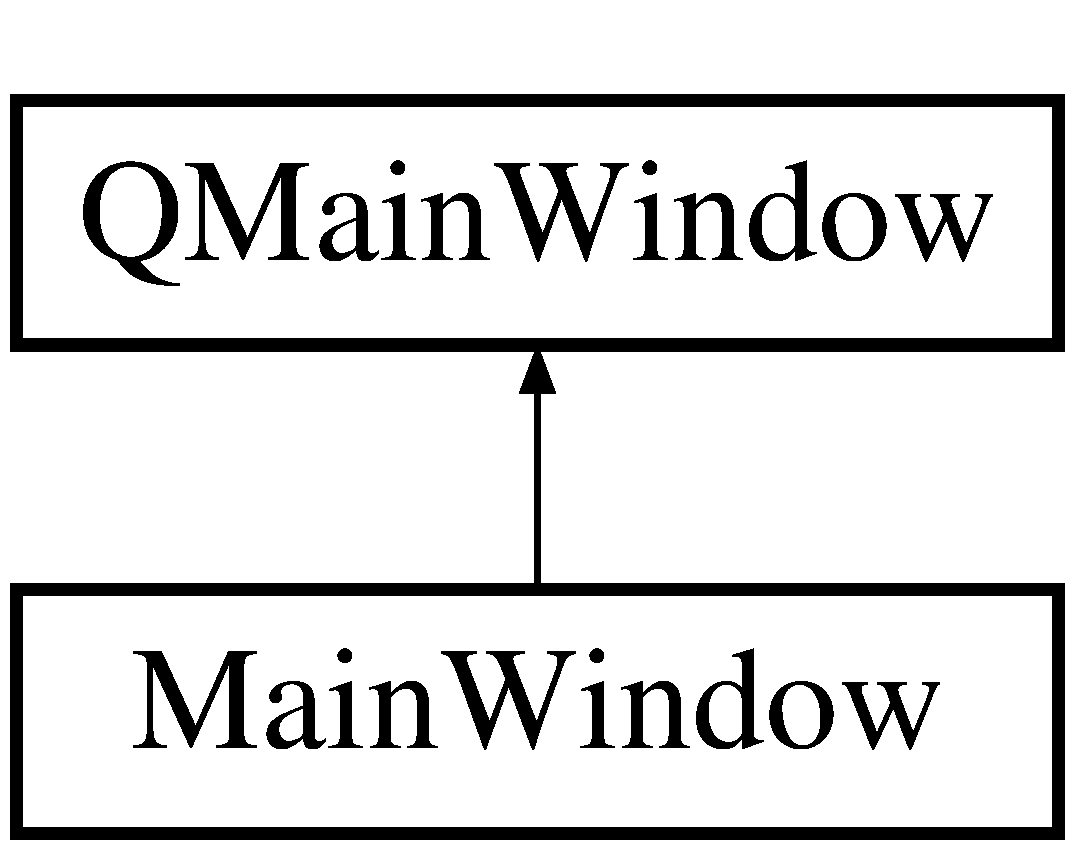
\includegraphics[height=2.000000cm]{class_main_window}
\end{center}
\end{figure}
\subsection*{Public Slots}
\begin{DoxyCompactItemize}
\item 
void \mbox{\hyperlink{class_main_window_a26b6030035e196b64333906db8302cdd}{tcp\+Connect}} (void)
\begin{DoxyCompactList}\small\item\em Realiza conexão com o server. \end{DoxyCompactList}\item 
void \mbox{\hyperlink{class_main_window_a3389bbbe4222f115a7609037a1a63bd5}{tcp\+Disconnect}} (void)
\begin{DoxyCompactList}\small\item\em Desconecta do server. \end{DoxyCompactList}\item 
void \mbox{\hyperlink{class_main_window_ac6d3a5fa8ef8ede69436b9e9a6ee80c1}{get\+Data}} (void)
\begin{DoxyCompactList}\small\item\em Captura dados do servidor de acordo com o tempo determinado pelo user. \end{DoxyCompactList}\item 
void \mbox{\hyperlink{class_main_window_a2e3dceeb08f18cc1d07e42b79fe7a0c1}{stop\+Data}} (void)
\begin{DoxyCompactList}\small\item\em Para a captura de dados. \end{DoxyCompactList}\item 
void \mbox{\hyperlink{class_main_window_a6d5ab019a97676b4edfe7d4b6a541455}{update\+Ip}} (void)
\begin{DoxyCompactList}\small\item\em Mostra uma lista dos clientes conectados. \end{DoxyCompactList}\item 
void \mbox{\hyperlink{class_main_window_a9d08a694a5f9c532225754381b8011ea}{timer\+Event}} (Q\+Timer\+Event $\ast$e)
\begin{DoxyCompactList}\small\item\em Função que determina o tempo da captura de dados definido pelo user. \end{DoxyCompactList}\end{DoxyCompactItemize}
\subsection*{Public Member Functions}
\begin{DoxyCompactItemize}
\item 
\mbox{\hyperlink{class_main_window_a8b244be8b7b7db1b08de2a2acb9409db}{Main\+Window}} (Q\+Widget $\ast$parent=0)
\item 
\mbox{\hyperlink{class_main_window_ae98d00a93bc118200eeef9f9bba1dba7}{$\sim$\+Main\+Window}} ()
\end{DoxyCompactItemize}


\subsection{Constructor \& Destructor Documentation}
\mbox{\Hypertarget{class_main_window_a8b244be8b7b7db1b08de2a2acb9409db}\label{class_main_window_a8b244be8b7b7db1b08de2a2acb9409db}} 
\index{Main\+Window@{Main\+Window}!Main\+Window@{Main\+Window}}
\index{Main\+Window@{Main\+Window}!Main\+Window@{Main\+Window}}
\subsubsection{\texorpdfstring{Main\+Window()}{MainWindow()}}
{\footnotesize\ttfamily Main\+Window\+::\+Main\+Window (\begin{DoxyParamCaption}\item[{Q\+Widget $\ast$}]{parent = {\ttfamily 0} }\end{DoxyParamCaption})\hspace{0.3cm}{\ttfamily [explicit]}}


\begin{DoxyCode}
13                                       :
14     QMainWindow(parent),
15     ui(\textcolor{keyword}{new} Ui::MainWindow)
16 \{
17     ui->setupUi(\textcolor{keyword}{this});
18     socket = \textcolor{keyword}{new} QTcpSocket(\textcolor{keyword}{this});
19     idTimer = 0;
20 
21     connect(ui->pushButtonGet,
22             SIGNAL(clicked(\textcolor{keywordtype}{bool})),
23             \textcolor{keyword}{this},
24             SLOT(\mbox{\hyperlink{class_main_window_ac6d3a5fa8ef8ede69436b9e9a6ee80c1}{getData}}()));
25     connect(ui->pushButton\_Stop,
26             SIGNAL(clicked(\textcolor{keywordtype}{bool})),
27             \textcolor{keyword}{this},
28             SLOT(\mbox{\hyperlink{class_main_window_a2e3dceeb08f18cc1d07e42b79fe7a0c1}{stopData}}()));
29     connect(ui->pushButton\_Connect,
30             SIGNAL(clicked(\textcolor{keywordtype}{bool})),
31             \textcolor{keyword}{this},
32             SLOT(\mbox{\hyperlink{class_main_window_a26b6030035e196b64333906db8302cdd}{tcpConnect}}()));
33     connect(ui->pushButton\_Disconnect,
34             SIGNAL(clicked(\textcolor{keywordtype}{bool})),
35             \textcolor{keyword}{this},
36             SLOT(\mbox{\hyperlink{class_main_window_a3389bbbe4222f115a7609037a1a63bd5}{tcpDisconnect}}()));
37     connect(ui->pushButton\_Update,
38             SIGNAL(clicked(\textcolor{keywordtype}{bool})),
39             \textcolor{keyword}{this},
40             SLOT(\mbox{\hyperlink{class_main_window_a6d5ab019a97676b4edfe7d4b6a541455}{updateIp}}()));
41 \}
\end{DoxyCode}
\mbox{\Hypertarget{class_main_window_ae98d00a93bc118200eeef9f9bba1dba7}\label{class_main_window_ae98d00a93bc118200eeef9f9bba1dba7}} 
\index{Main\+Window@{Main\+Window}!````~Main\+Window@{$\sim$\+Main\+Window}}
\index{````~Main\+Window@{$\sim$\+Main\+Window}!Main\+Window@{Main\+Window}}
\subsubsection{\texorpdfstring{$\sim$\+Main\+Window()}{~MainWindow()}}
{\footnotesize\ttfamily Main\+Window\+::$\sim$\+Main\+Window (\begin{DoxyParamCaption}{ }\end{DoxyParamCaption})}


\begin{DoxyCode}
170 \{
171     \textcolor{keyword}{delete} socket;
172     \textcolor{keyword}{delete} ui;
173 \}
\end{DoxyCode}


\subsection{Member Function Documentation}
\mbox{\Hypertarget{class_main_window_ac6d3a5fa8ef8ede69436b9e9a6ee80c1}\label{class_main_window_ac6d3a5fa8ef8ede69436b9e9a6ee80c1}} 
\index{Main\+Window@{Main\+Window}!get\+Data@{get\+Data}}
\index{get\+Data@{get\+Data}!Main\+Window@{Main\+Window}}
\subsubsection{\texorpdfstring{get\+Data}{getData}}
{\footnotesize\ttfamily void Main\+Window\+::get\+Data (\begin{DoxyParamCaption}\item[{void}]{ }\end{DoxyParamCaption})\hspace{0.3cm}{\ttfamily [slot]}}



Captura dados do servidor de acordo com o tempo determinado pelo user. 


\begin{DoxyCode}
58                         \{
59     \textcolor{keywordflow}{if}(idTimer)\{
60         killTimer(idTimer);
61     \}
62     idTimer = startTimer(ui->horizontalSlider\_Time->value()*1000);
63 
64 \}
\end{DoxyCode}
\mbox{\Hypertarget{class_main_window_a2e3dceeb08f18cc1d07e42b79fe7a0c1}\label{class_main_window_a2e3dceeb08f18cc1d07e42b79fe7a0c1}} 
\index{Main\+Window@{Main\+Window}!stop\+Data@{stop\+Data}}
\index{stop\+Data@{stop\+Data}!Main\+Window@{Main\+Window}}
\subsubsection{\texorpdfstring{stop\+Data}{stopData}}
{\footnotesize\ttfamily void Main\+Window\+::stop\+Data (\begin{DoxyParamCaption}\item[{void}]{ }\end{DoxyParamCaption})\hspace{0.3cm}{\ttfamily [slot]}}



Para a captura de dados. 


\begin{DoxyCode}
143                              \{
144     \textcolor{keywordflow}{if}(idTimer)\{
145         killTimer(idTimer);
146     \}
147 \}
\end{DoxyCode}
\mbox{\Hypertarget{class_main_window_a26b6030035e196b64333906db8302cdd}\label{class_main_window_a26b6030035e196b64333906db8302cdd}} 
\index{Main\+Window@{Main\+Window}!tcp\+Connect@{tcp\+Connect}}
\index{tcp\+Connect@{tcp\+Connect}!Main\+Window@{Main\+Window}}
\subsubsection{\texorpdfstring{tcp\+Connect}{tcpConnect}}
{\footnotesize\ttfamily void Main\+Window\+::tcp\+Connect (\begin{DoxyParamCaption}\item[{void}]{ }\end{DoxyParamCaption})\hspace{0.3cm}{\ttfamily [slot]}}



Realiza conexão com o server. 


\begin{DoxyCode}
43                            \{
44     socket->connectToHost(ui->lineEdit\_Host->text(),1234);
45     \textcolor{keywordflow}{if}(socket->waitForConnected())\{
46         qDebug() << \textcolor{stringliteral}{"Connected"};
47     \}
48     \textcolor{keywordflow}{else}\{
49         qDebug() << \textcolor{stringliteral}{"Disconnected"};
50     \}
51 \}
\end{DoxyCode}
\mbox{\Hypertarget{class_main_window_a3389bbbe4222f115a7609037a1a63bd5}\label{class_main_window_a3389bbbe4222f115a7609037a1a63bd5}} 
\index{Main\+Window@{Main\+Window}!tcp\+Disconnect@{tcp\+Disconnect}}
\index{tcp\+Disconnect@{tcp\+Disconnect}!Main\+Window@{Main\+Window}}
\subsubsection{\texorpdfstring{tcp\+Disconnect}{tcpDisconnect}}
{\footnotesize\ttfamily void Main\+Window\+::tcp\+Disconnect (\begin{DoxyParamCaption}\item[{void}]{ }\end{DoxyParamCaption})\hspace{0.3cm}{\ttfamily [slot]}}



Desconecta do server. 


\begin{DoxyCode}
53                               \{
54     socket->disconnectFromHost();
55 \}
\end{DoxyCode}
\mbox{\Hypertarget{class_main_window_a9d08a694a5f9c532225754381b8011ea}\label{class_main_window_a9d08a694a5f9c532225754381b8011ea}} 
\index{Main\+Window@{Main\+Window}!timer\+Event@{timer\+Event}}
\index{timer\+Event@{timer\+Event}!Main\+Window@{Main\+Window}}
\subsubsection{\texorpdfstring{timer\+Event}{timerEvent}}
{\footnotesize\ttfamily void Main\+Window\+::timer\+Event (\begin{DoxyParamCaption}\item[{Q\+Timer\+Event $\ast$}]{e }\end{DoxyParamCaption})\hspace{0.3cm}{\ttfamily [slot]}}



Função que determina o tempo da captura de dados definido pelo user. 


\begin{DoxyCode}
66                                          \{
67     QString str;
68     QStringList list;
69     qint64 thetime, num;
70     \textcolor{keywordtype}{double} max\_x, min\_x, min\_y, max\_y;
71     std::vector<double> time;
72     std::vector<double> data;
73     std::vector<double> temposnorm;
74     std::vector<double> dadosnorm;
75 
76     qDebug() << \textcolor{stringliteral}{"to get data..."};
77     \textcolor{keywordflow}{if}(socket->state() == QAbstractSocket::ConnectedState)\{
78         \textcolor{keywordflow}{if}(socket->isOpen())\{
79             qDebug() << \textcolor{stringliteral}{"reading..."};
80             str = \textcolor{stringliteral}{"get "} + ui->listWidget\_ListaDeClients->currentItem()->text() + \textcolor{stringliteral}{" 30\(\backslash\)r\(\backslash\)n"};
81             socket->write(str.toStdString().c\_str());
82             socket->waitForBytesWritten();
83             socket->waitForReadyRead();
84             qDebug() << socket->bytesAvailable();
85             time.clear();
86             data.clear();
87             \textcolor{keywordflow}{while}(socket->bytesAvailable())\{
88                 str = socket->readLine().replace(\textcolor{stringliteral}{"\(\backslash\)n"},\textcolor{stringliteral}{""}).replace(\textcolor{stringliteral}{"\(\backslash\)r"},\textcolor{stringliteral}{""});
89                 list = str.split(\textcolor{stringliteral}{" "});
90 
91                 \textcolor{keywordflow}{if}(list.size() == 2)\{
92                     \textcolor{keywordtype}{bool} ok;
93                     str = list.at(0);
94                     thetime = str.toLongLong(&ok);
95                     time.push\_back(thetime);
96 
97                     str = list.at(1);
98                     num = str.toLongLong(&ok);
99                     data.push\_back(num);
100                     qDebug() << thetime << \textcolor{stringliteral}{": "} << str;
101                 \}
102             \}
103         \}
104     \}
105 
106     qDebug()<<data.size()<<time.size();
107     \textcolor{comment}{//achando valores maximos e minimos}
108     max\_x = time[0], min\_x = time[0];
109     min\_y = data[0], max\_y = data[0];
110 
111     \textcolor{keywordflow}{for}(\textcolor{keywordtype}{int} i = 1 ; i < 30; i++)\{
112         \textcolor{keywordflow}{if}(time[i] < min\_x)\{
113             min\_x = time[i];
114         \}
115         \textcolor{keywordflow}{else} \textcolor{keywordflow}{if}(time[i] > max\_x)\{
116             max\_x = time[i];
117         \}
118         \textcolor{keywordflow}{if}(data[i] < min\_y)\{
119             min\_y = data[i];
120         \}
121         \textcolor{keywordflow}{else} \textcolor{keywordflow}{if}(data[i] > max\_y)\{
122             max\_y = data[i];
123         \}
124     \}
125 
126     qDebug()<<max\_x-min\_x;
127 
128 
129     qDebug()<<max\_y<<min\_y;
130 
131 
132     \textcolor{comment}{//normalizando dados}
133     temposnorm.clear();
134     dadosnorm.clear();
135     \textcolor{keywordflow}{for}(\textcolor{keywordtype}{int} i = 0; i<30; i++)\{
136         temposnorm.push\_back((time[i] - min\_x)/(max\_x - min\_x));
137         dadosnorm.push\_back((data[i] - min\_y)/(max\_y - min\_y));
138     \}
139     qDebug()<<\textcolor{stringliteral}{"passou"};
140     ui->widget\_Plotter->loadData(temposnorm,dadosnorm);
141 \}
\end{DoxyCode}
\mbox{\Hypertarget{class_main_window_a6d5ab019a97676b4edfe7d4b6a541455}\label{class_main_window_a6d5ab019a97676b4edfe7d4b6a541455}} 
\index{Main\+Window@{Main\+Window}!update\+Ip@{update\+Ip}}
\index{update\+Ip@{update\+Ip}!Main\+Window@{Main\+Window}}
\subsubsection{\texorpdfstring{update\+Ip}{updateIp}}
{\footnotesize\ttfamily void Main\+Window\+::update\+Ip (\begin{DoxyParamCaption}\item[{void}]{ }\end{DoxyParamCaption})\hspace{0.3cm}{\ttfamily [slot]}}



Mostra uma lista dos clientes conectados. 


\begin{DoxyCode}
149                              \{
150     QString str;
151 
152     ui->listWidget\_ListaDeClients->clear();
153     \textcolor{keywordflow}{if}(socket->state() == QAbstractSocket::ConnectedState)\{
154         socket->write(\textcolor{stringliteral}{"list\(\backslash\)r\(\backslash\)n"});
155         socket->waitForBytesWritten();
156         socket->waitForReadyRead();
157         \textcolor{keywordflow}{while}(socket->bytesAvailable())\{
158             str = socket->readLine().replace(\textcolor{stringliteral}{"\(\backslash\)n"},\textcolor{stringliteral}{""}).replace(\textcolor{stringliteral}{"\(\backslash\)r"},\textcolor{stringliteral}{""});
159             ui->listWidget\_ListaDeClients->addItem(str);
160         \}
161     \}
162     \textcolor{keywordflow}{else}\{
163         ui->listWidget\_ListaDeClients->addItem(\textcolor{stringliteral}{"Lista vazia"});
164     \}
165 
166 \}
\end{DoxyCode}


The documentation for this class was generated from the following files\+:\begin{DoxyCompactItemize}
\item 
C\+:/\+Users/mateu/\+Documents/\+Cliente\+\_\+\+Consumidor/\mbox{\hyperlink{mainwindow_8h}{mainwindow.\+h}}\item 
C\+:/\+Users/mateu/\+Documents/\+Cliente\+\_\+\+Consumidor/\mbox{\hyperlink{mainwindow_8cpp}{mainwindow.\+cpp}}\end{DoxyCompactItemize}

\hypertarget{class_ui_1_1_main_window}{}\section{Referência da Classe Ui\+:\+:Main\+Window}
\label{class_ui_1_1_main_window}\index{Ui\+::\+Main\+Window@{Ui\+::\+Main\+Window}}


{\ttfamily \#include $<$ui\+\_\+mainwindow.\+h$>$}

Diagrama de hierarquia para Ui\+:\+:Main\+Window\+:\begin{figure}[H]
\begin{center}
\leavevmode
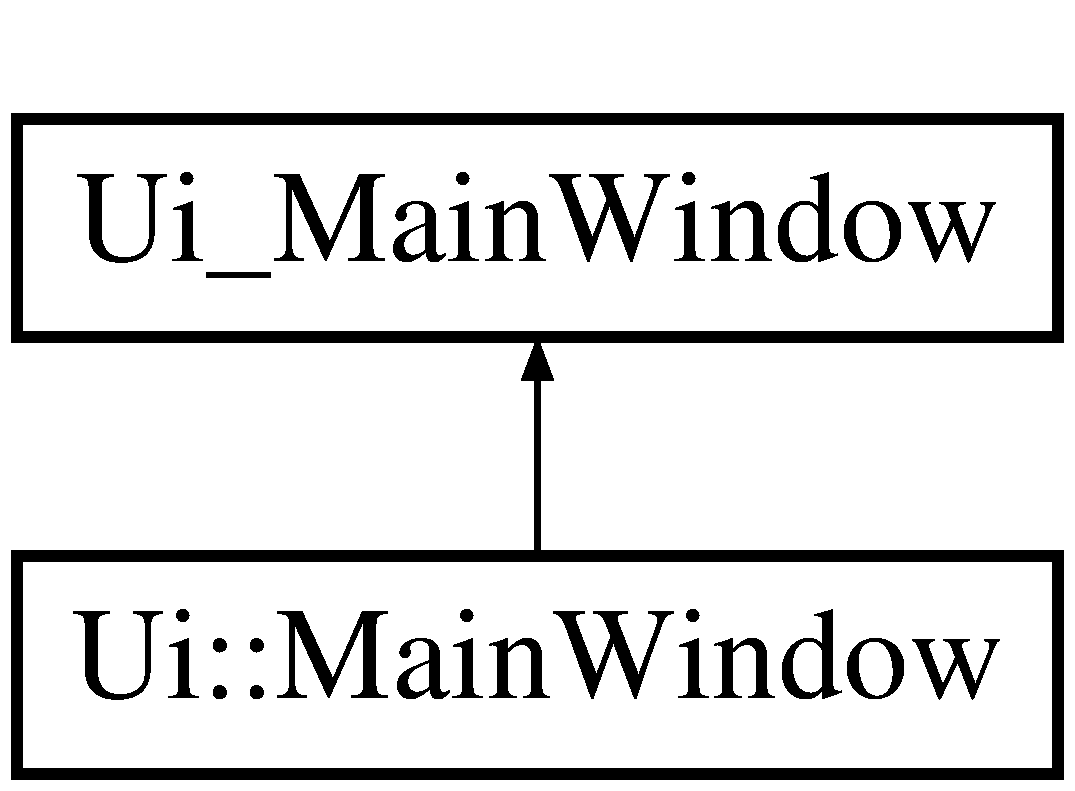
\includegraphics[height=2.000000cm]{class_ui_1_1_main_window}
\end{center}
\end{figure}
\subsection*{Outros membros herdados}


A documentação para essa classe foi gerada a partir do seguinte arquivo\+:\begin{DoxyCompactItemize}
\item 
C\+:/\+Users/mateu/\+Documents/\+Projeto Final D\+C\+A 1202/\+Qt\+Tcp\+Server/\mbox{\hyperlink{ui__mainwindow_8h}{ui\+\_\+mainwindow.\+h}}\end{DoxyCompactItemize}

\hypertarget{class_my_server}{}\section{Referência da Classe My\+Server}
\label{class_my_server}\index{My\+Server@{My\+Server}}


The \mbox{\hyperlink{class_my_server}{My\+Server}} class inicia um servidor T\+CP capaz de \char`\"{}ouvir\char`\"{} a porta 1234.  




{\ttfamily \#include $<$myserver.\+h$>$}

Diagrama de hierarquia para My\+Server\+:\begin{figure}[H]
\begin{center}
\leavevmode
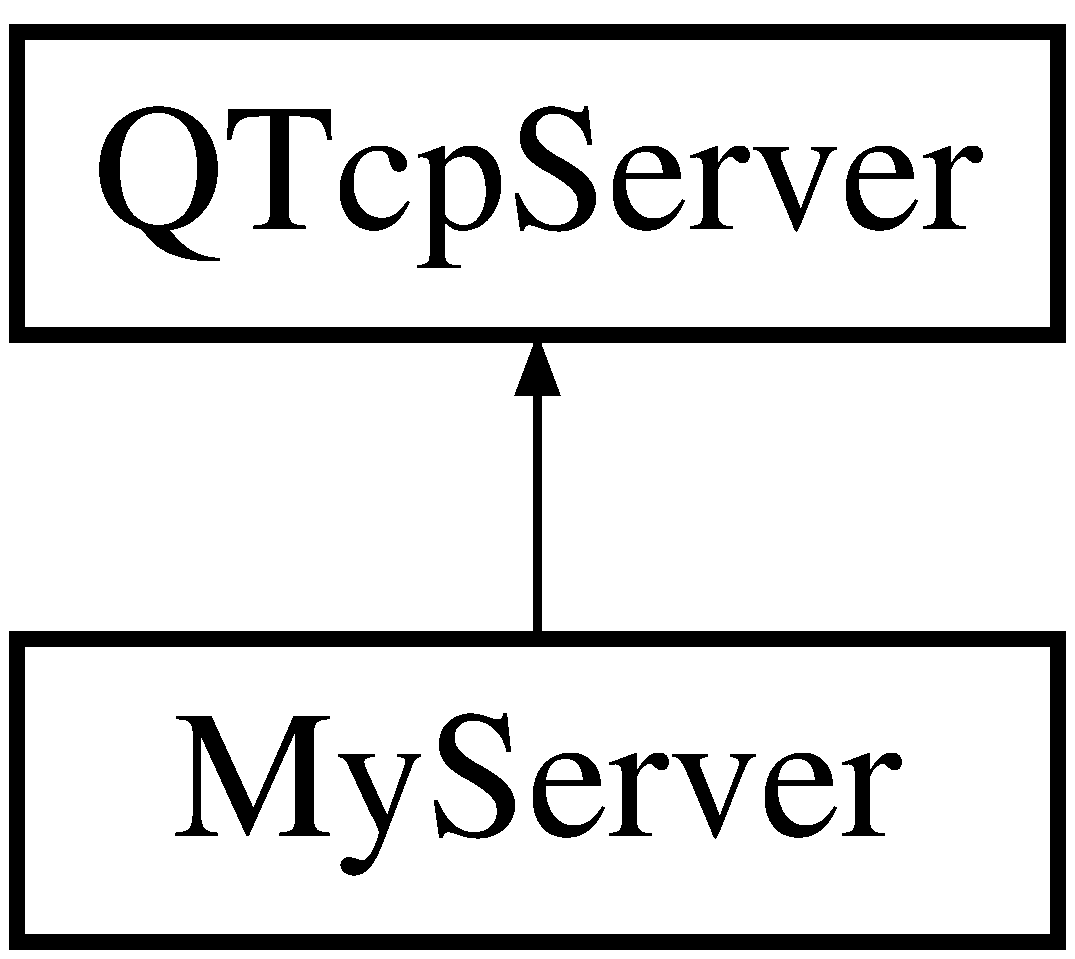
\includegraphics[height=2.000000cm]{class_my_server}
\end{center}
\end{figure}
\subsection*{Slots Públicos}
\begin{DoxyCompactItemize}
\item 
void \mbox{\hyperlink{class_my_server_ac795ee6f1607c0fa4e635a0da2bf2164}{receive\+Msg}} (Q\+String str)
\end{DoxyCompactItemize}
\subsection*{Sinais}
\begin{DoxyCompactItemize}
\item 
void \mbox{\hyperlink{class_my_server_a2b884bce37840b1b461363a37b463b30}{message}} (Q\+String)
\end{DoxyCompactItemize}
\subsection*{Membros Públicos}
\begin{DoxyCompactItemize}
\item 
\mbox{\hyperlink{class_my_server_ac9e5ca7b551a5df90d5b39260f7e5404}{My\+Server}} (Q\+Object $\ast$parent=0)
\begin{DoxyCompactList}\small\item\em \mbox{\hyperlink{class_my_server}{My\+Server}} é o construtor da classe. \end{DoxyCompactList}\item 
void \mbox{\hyperlink{class_my_server_a962f0e205a0aaf08b12d50d1315a8c90}{start\+Server}} ()
\begin{DoxyCompactList}\small\item\em Start\+Server start the T\+CP server. \end{DoxyCompactList}\item 
Q\+String\+List \mbox{\hyperlink{class_my_server_ac10d498dcc2b5d691f131f17b6602a59}{get\+I\+P\+List}} ()
\begin{DoxyCompactList}\small\item\em get\+I\+P\+List return a list of I\+Ps used by server \end{DoxyCompactList}\end{DoxyCompactItemize}
\subsection*{Membros Protegidos}
\begin{DoxyCompactItemize}
\item 
void \mbox{\hyperlink{class_my_server_a635c7a1e6817285ffb1a2a3842df010b}{incoming\+Connection}} (qintptr socket\+Descriptor)
\begin{DoxyCompactList}\small\item\em incoming\+Connection decide o que fazer quando uma nova conexao é iniciada \end{DoxyCompactList}\end{DoxyCompactItemize}


\subsection{Descrição detalhada}
The \mbox{\hyperlink{class_my_server}{My\+Server}} class inicia um servidor T\+CP capaz de \char`\"{}ouvir\char`\"{} a porta 1234. 

\subsection{Construtores e Destrutores}
\mbox{\Hypertarget{class_my_server_ac9e5ca7b551a5df90d5b39260f7e5404}\label{class_my_server_ac9e5ca7b551a5df90d5b39260f7e5404}} 
\index{My\+Server@{My\+Server}!My\+Server@{My\+Server}}
\index{My\+Server@{My\+Server}!My\+Server@{My\+Server}}
\subsubsection{\texorpdfstring{My\+Server()}{MyServer()}}
{\footnotesize\ttfamily My\+Server\+::\+My\+Server (\begin{DoxyParamCaption}\item[{Q\+Object $\ast$}]{parent = {\ttfamily 0} }\end{DoxyParamCaption})}



\mbox{\hyperlink{class_my_server}{My\+Server}} é o construtor da classe. 


\begin{DoxyParams}{Parâmetros}
{\em parent} & eh o pai do objeto (nao usado) \\
\hline
\end{DoxyParams}

\begin{DoxyCode}
3                                   :
4   QTcpServer(parent)
5 \{
6 
7 \}
\end{DoxyCode}


\subsection{Funções membros}
\mbox{\Hypertarget{class_my_server_ac10d498dcc2b5d691f131f17b6602a59}\label{class_my_server_ac10d498dcc2b5d691f131f17b6602a59}} 
\index{My\+Server@{My\+Server}!get\+I\+P\+List@{get\+I\+P\+List}}
\index{get\+I\+P\+List@{get\+I\+P\+List}!My\+Server@{My\+Server}}
\subsubsection{\texorpdfstring{get\+I\+P\+List()}{getIPList()}}
{\footnotesize\ttfamily Q\+String\+List My\+Server\+::get\+I\+P\+List (\begin{DoxyParamCaption}{ }\end{DoxyParamCaption})}



get\+I\+P\+List return a list of I\+Ps used by server 

\begin{DoxyReturn}{Retorna}

\end{DoxyReturn}

\begin{DoxyCode}
22                                \{
23   \textcolor{keywordflow}{return} iplist;
24 \}
\end{DoxyCode}
\mbox{\Hypertarget{class_my_server_a635c7a1e6817285ffb1a2a3842df010b}\label{class_my_server_a635c7a1e6817285ffb1a2a3842df010b}} 
\index{My\+Server@{My\+Server}!incoming\+Connection@{incoming\+Connection}}
\index{incoming\+Connection@{incoming\+Connection}!My\+Server@{My\+Server}}
\subsubsection{\texorpdfstring{incoming\+Connection()}{incomingConnection()}}
{\footnotesize\ttfamily void My\+Server\+::incoming\+Connection (\begin{DoxyParamCaption}\item[{qintptr}]{socket\+Descriptor }\end{DoxyParamCaption})\hspace{0.3cm}{\ttfamily [protected]}}



incoming\+Connection decide o que fazer quando uma nova conexao é iniciada 


\begin{DoxyParams}{Parâmetros}
{\em socket\+Descriptor} & é o identificador do socket para a conexao \\
\hline
\end{DoxyParams}

\begin{DoxyCode}
30                                                          \{
31   QString str;
32   str = QString(\textcolor{stringliteral}{"<i>"}) + QString().setNum(socketDescriptor) +
33       \textcolor{stringliteral}{" connecting...</i>"};
34   emit \mbox{\hyperlink{class_my_server_a2b884bce37840b1b461363a37b463b30}{message}}(str);
35   \mbox{\hyperlink{class_my_thread}{MyThread}} *thread = \textcolor{keyword}{new} \mbox{\hyperlink{class_my_thread}{MyThread}}(socketDescriptor,\textcolor{keyword}{this}, &storage);
36   \textcolor{comment}{// assegura que o objeto da thread será deletado quando a thread}
37   \textcolor{comment}{// for finalizada.}
38   connect(thread,SIGNAL(finished()), thread, SLOT(deleteLater()));
39 
40   \textcolor{comment}{// redireciona as mensagens enviadas pela thread para serem reemitidos}
41   \textcolor{comment}{// pelo servidor}
42   connect(thread,SIGNAL(\mbox{\hyperlink{class_my_server_a2b884bce37840b1b461363a37b463b30}{message}}(QString)), \textcolor{keyword}{this}, SLOT(\mbox{\hyperlink{class_my_server_ac795ee6f1607c0fa4e635a0da2bf2164}{receiveMsg}}(QString)));
43   thread->\mbox{\hyperlink{class_my_thread_a48f2e366e852087c53705f64e1ee65c2}{run}}();
44 \}
\end{DoxyCode}
\mbox{\Hypertarget{class_my_server_a2b884bce37840b1b461363a37b463b30}\label{class_my_server_a2b884bce37840b1b461363a37b463b30}} 
\index{My\+Server@{My\+Server}!message@{message}}
\index{message@{message}!My\+Server@{My\+Server}}
\subsubsection{\texorpdfstring{message}{message}}
{\footnotesize\ttfamily void My\+Server\+::message (\begin{DoxyParamCaption}\item[{Q\+String}]{\+\_\+t1 }\end{DoxyParamCaption})\hspace{0.3cm}{\ttfamily [signal]}}


\begin{DoxyCode}
132 \{
133     \textcolor{keywordtype}{void} *\_a[] = \{ Q\_NULLPTR, \textcolor{keyword}{const\_cast<}\textcolor{keywordtype}{void}*\textcolor{keyword}{>}(\textcolor{keyword}{reinterpret\_cast<}\textcolor{keyword}{const }\textcolor{keywordtype}{void}*\textcolor{keyword}{>}(&\_t1)) \};
134     QMetaObject::activate(\textcolor{keyword}{this}, &staticMetaObject, 0, \_a);
135 \}
\end{DoxyCode}
\mbox{\Hypertarget{class_my_server_ac795ee6f1607c0fa4e635a0da2bf2164}\label{class_my_server_ac795ee6f1607c0fa4e635a0da2bf2164}} 
\index{My\+Server@{My\+Server}!receive\+Msg@{receive\+Msg}}
\index{receive\+Msg@{receive\+Msg}!My\+Server@{My\+Server}}
\subsubsection{\texorpdfstring{receive\+Msg}{receiveMsg}}
{\footnotesize\ttfamily void My\+Server\+::receive\+Msg (\begin{DoxyParamCaption}\item[{Q\+String}]{str }\end{DoxyParamCaption})\hspace{0.3cm}{\ttfamily [slot]}}


\begin{DoxyCode}
26                                     \{
27   emit \mbox{\hyperlink{class_my_server_a2b884bce37840b1b461363a37b463b30}{message}}(str);
28 \}
\end{DoxyCode}
\mbox{\Hypertarget{class_my_server_a962f0e205a0aaf08b12d50d1315a8c90}\label{class_my_server_a962f0e205a0aaf08b12d50d1315a8c90}} 
\index{My\+Server@{My\+Server}!start\+Server@{start\+Server}}
\index{start\+Server@{start\+Server}!My\+Server@{My\+Server}}
\subsubsection{\texorpdfstring{start\+Server()}{startServer()}}
{\footnotesize\ttfamily void My\+Server\+::start\+Server (\begin{DoxyParamCaption}{ }\end{DoxyParamCaption})}



Start\+Server start the T\+CP server. 


\begin{DoxyCode}
9                           \{
10   \textcolor{keywordflow}{if}(!this->listen(QHostAddress::Any, 1234))\{
11     emit \mbox{\hyperlink{class_my_server_a2b884bce37840b1b461363a37b463b30}{message}}(QString(\textcolor{stringliteral}{"<b>server did not start!</b>"}));
12   \}
13   \textcolor{keywordflow}{else}\{
14     emit \mbox{\hyperlink{class_my_server_a2b884bce37840b1b461363a37b463b30}{message}}(QString(\textcolor{stringliteral}{"<b>server started!</b>"}));
15     \textcolor{keywordflow}{foreach} (\textcolor{keyword}{const} QHostAddress &address, QNetworkInterface::allAddresses()) \{
16       \textcolor{keywordflow}{if} (address.protocol() == QAbstractSocket::IPv4Protocol && address != QHostAddress(
      QHostAddress::LocalHost))
17         iplist << address.toString();
18     \}
19   \}
20 \}
\end{DoxyCode}


A documentação para essa classe foi gerada a partir dos seguintes arquivos\+:\begin{DoxyCompactItemize}
\item 
C\+:/\+Users/mateu/\+Documents/\+Projeto Final D\+C\+A 1202/\+Qt\+Tcp\+Server/\mbox{\hyperlink{myserver_8h}{myserver.\+h}}\item 
C\+:/\+Users/mateu/\+Documents/\+Projeto Final D\+C\+A 1202/\+Qt\+Tcp\+Server/\mbox{\hyperlink{moc__myserver_8cpp}{moc\+\_\+myserver.\+cpp}}\item 
C\+:/\+Users/mateu/\+Documents/\+Projeto Final D\+C\+A 1202/\+Qt\+Tcp\+Server/\mbox{\hyperlink{myserver_8cpp}{myserver.\+cpp}}\end{DoxyCompactItemize}

\hypertarget{class_my_thread}{}\section{Referência da Classe My\+Thread}
\label{class_my_thread}\index{My\+Thread@{My\+Thread}}


The \mbox{\hyperlink{class_my_thread}{My\+Thread}} class cria uma thread que lida com o tratamento de uma conexao T\+CP de entrada.  




{\ttfamily \#include $<$mythread.\+h$>$}

Diagrama de hierarquia para My\+Thread\+:\begin{figure}[H]
\begin{center}
\leavevmode
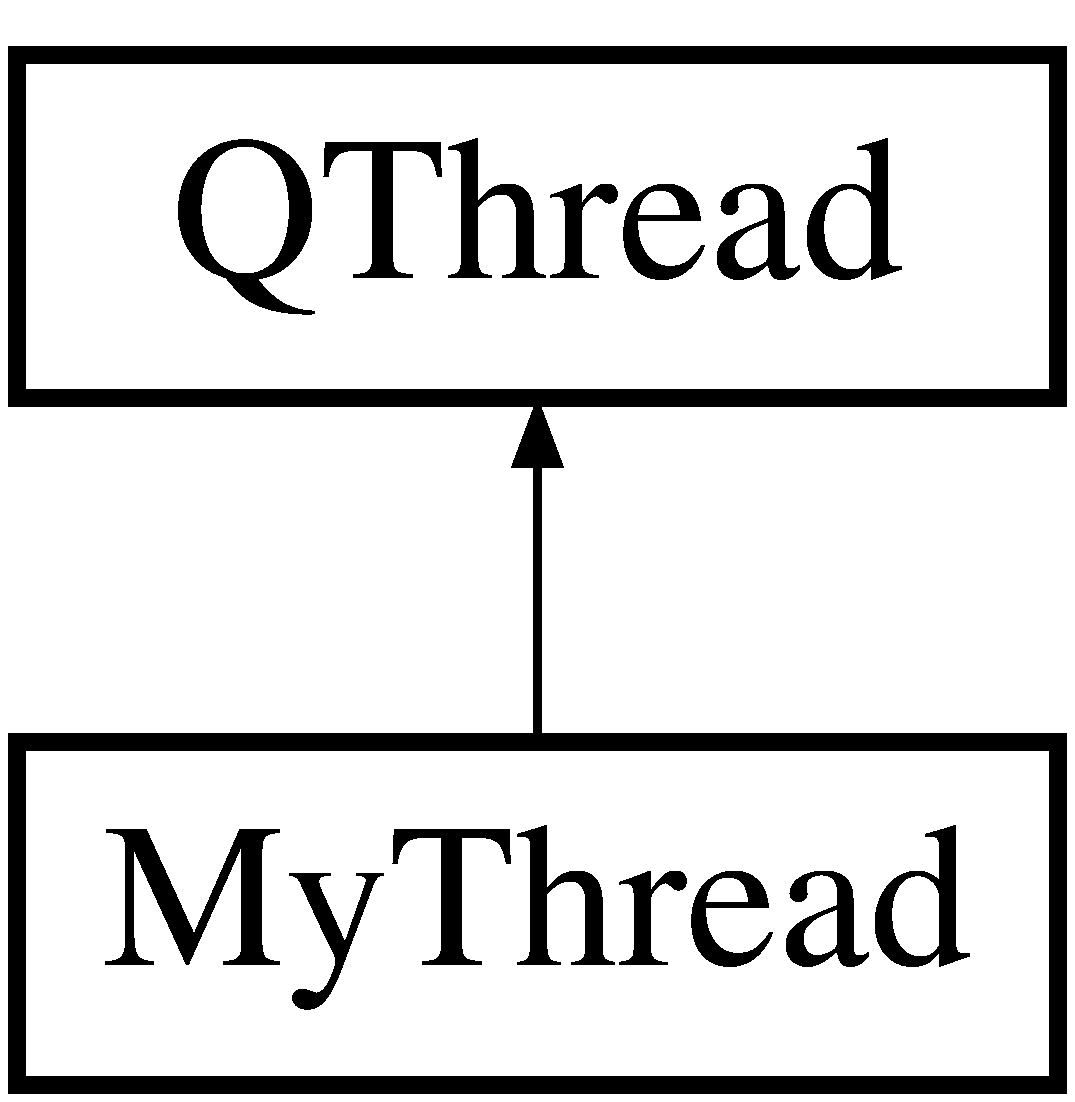
\includegraphics[height=2.000000cm]{class_my_thread}
\end{center}
\end{figure}
\subsection*{Slots Públicos}
\begin{DoxyCompactItemize}
\item 
void \mbox{\hyperlink{class_my_thread_a277618fdd448b927f2e250c2076fc176}{ready\+Read}} ()
\item 
void \mbox{\hyperlink{class_my_thread_a447710039787ae20134a9b572487840f}{disconnected}} ()
\end{DoxyCompactItemize}
\subsection*{Sinais}
\begin{DoxyCompactItemize}
\item 
void \mbox{\hyperlink{class_my_thread_aebf11d93838f22c9547d0c6aa97002be}{error}} (Q\+Tcp\+Socket\+::\+Socket\+Error socketerror)
\item 
void \mbox{\hyperlink{class_my_thread_ae49528d4ec1b2208240f707f5aa74adf}{message}} (Q\+String)
\end{DoxyCompactItemize}
\subsection*{Membros Públicos}
\begin{DoxyCompactItemize}
\item 
\mbox{\hyperlink{class_my_thread_ac1b04b0fa6b32038e810c7105ef762f6}{My\+Thread}} (int ID, Q\+Object $\ast$parent, \mbox{\hyperlink{class_data_storage}{Data\+Storage}} $\ast$storage)
\begin{DoxyCompactList}\small\item\em \mbox{\hyperlink{class_my_thread}{My\+Thread}} eh o construtor da classe. \end{DoxyCompactList}\item 
void \mbox{\hyperlink{class_my_thread_a48f2e366e852087c53705f64e1ee65c2}{run}} ()
\end{DoxyCompactItemize}


\subsection{Descrição detalhada}
The \mbox{\hyperlink{class_my_thread}{My\+Thread}} class cria uma thread que lida com o tratamento de uma conexao T\+CP de entrada. 

\subsection{Construtores e Destrutores}
\mbox{\Hypertarget{class_my_thread_ac1b04b0fa6b32038e810c7105ef762f6}\label{class_my_thread_ac1b04b0fa6b32038e810c7105ef762f6}} 
\index{My\+Thread@{My\+Thread}!My\+Thread@{My\+Thread}}
\index{My\+Thread@{My\+Thread}!My\+Thread@{My\+Thread}}
\subsubsection{\texorpdfstring{My\+Thread()}{MyThread()}}
{\footnotesize\ttfamily My\+Thread\+::\+My\+Thread (\begin{DoxyParamCaption}\item[{int}]{ID,  }\item[{Q\+Object $\ast$}]{parent,  }\item[{\mbox{\hyperlink{class_data_storage}{Data\+Storage}} $\ast$}]{storage }\end{DoxyParamCaption})}



\mbox{\hyperlink{class_my_thread}{My\+Thread}} eh o construtor da classe. 


\begin{DoxyParams}{Parâmetros}
{\em ID} & eh o identificador da thread \\
\hline
{\em parent} & \\
\hline
{\em storage} & \\
\hline
\end{DoxyParams}

\begin{DoxyCode}
6                                                                 :
7   QThread (parent)
8 \{
9   this->socketDescriptor = ID;
10   this->storage = storage;
11 \}
\end{DoxyCode}


\subsection{Funções membros}
\mbox{\Hypertarget{class_my_thread_a447710039787ae20134a9b572487840f}\label{class_my_thread_a447710039787ae20134a9b572487840f}} 
\index{My\+Thread@{My\+Thread}!disconnected@{disconnected}}
\index{disconnected@{disconnected}!My\+Thread@{My\+Thread}}
\subsubsection{\texorpdfstring{disconnected}{disconnected}}
{\footnotesize\ttfamily void My\+Thread\+::disconnected (\begin{DoxyParamCaption}{ }\end{DoxyParamCaption})\hspace{0.3cm}{\ttfamily [slot]}}


\begin{DoxyCode}
110                            \{
111   str = QString(\textcolor{stringliteral}{"<i>"}) + QString().setNum(socketDescriptor)+
112       \textcolor{stringliteral}{" <font color=\(\backslash\)"red\(\backslash\)">Disconnected</font></i>"};
113   emit \mbox{\hyperlink{class_my_thread_ae49528d4ec1b2208240f707f5aa74adf}{message}}(str);
114   socket->deleteLater();
115   \textcolor{comment}{// diz a thread para parar}
116   exit(0);
117 \}
\end{DoxyCode}
\mbox{\Hypertarget{class_my_thread_aebf11d93838f22c9547d0c6aa97002be}\label{class_my_thread_aebf11d93838f22c9547d0c6aa97002be}} 
\index{My\+Thread@{My\+Thread}!error@{error}}
\index{error@{error}!My\+Thread@{My\+Thread}}
\subsubsection{\texorpdfstring{error}{error}}
{\footnotesize\ttfamily void My\+Thread\+::error (\begin{DoxyParamCaption}\item[{Q\+Tcp\+Socket\+::\+Socket\+Error}]{socketerror }\end{DoxyParamCaption})\hspace{0.3cm}{\ttfamily [signal]}}


\begin{DoxyCode}
150 \{
151     \textcolor{keywordtype}{void} *\_a[] = \{ Q\_NULLPTR, \textcolor{keyword}{const\_cast<}\textcolor{keywordtype}{void}*\textcolor{keyword}{>}(\textcolor{keyword}{reinterpret\_cast<}\textcolor{keyword}{const }\textcolor{keywordtype}{void}*\textcolor{keyword}{>}(&\_t1)) \};
152     QMetaObject::activate(\textcolor{keyword}{this}, &staticMetaObject, 0, \_a);
153 \}
\end{DoxyCode}
\mbox{\Hypertarget{class_my_thread_ae49528d4ec1b2208240f707f5aa74adf}\label{class_my_thread_ae49528d4ec1b2208240f707f5aa74adf}} 
\index{My\+Thread@{My\+Thread}!message@{message}}
\index{message@{message}!My\+Thread@{My\+Thread}}
\subsubsection{\texorpdfstring{message}{message}}
{\footnotesize\ttfamily void My\+Thread\+::message (\begin{DoxyParamCaption}\item[{Q\+String}]{\+\_\+t1 }\end{DoxyParamCaption})\hspace{0.3cm}{\ttfamily [signal]}}


\begin{DoxyCode}
157 \{
158     \textcolor{keywordtype}{void} *\_a[] = \{ Q\_NULLPTR, \textcolor{keyword}{const\_cast<}\textcolor{keywordtype}{void}*\textcolor{keyword}{>}(\textcolor{keyword}{reinterpret\_cast<}\textcolor{keyword}{const }\textcolor{keywordtype}{void}*\textcolor{keyword}{>}(&\_t1)) \};
159     QMetaObject::activate(\textcolor{keyword}{this}, &staticMetaObject, 1, \_a);
160 \}
\end{DoxyCode}
\mbox{\Hypertarget{class_my_thread_a277618fdd448b927f2e250c2076fc176}\label{class_my_thread_a277618fdd448b927f2e250c2076fc176}} 
\index{My\+Thread@{My\+Thread}!ready\+Read@{ready\+Read}}
\index{ready\+Read@{ready\+Read}!My\+Thread@{My\+Thread}}
\subsubsection{\texorpdfstring{ready\+Read}{readyRead}}
{\footnotesize\ttfamily void My\+Thread\+::ready\+Read (\begin{DoxyParamCaption}{ }\end{DoxyParamCaption})\hspace{0.3cm}{\ttfamily [slot]}}


\begin{DoxyCode}
35                         \{
36   vector<Entry> entry;
37   vector<QHostAddress> hostList;
38   \mbox{\hyperlink{struct_entry}{Entry}} value;
39   qint64 msecdate;
40   \textcolor{keywordtype}{unsigned} \textcolor{keywordtype}{int} nsamples;
41   QString cmd;
42 
43   QString str = socket->readLine().replace(\textcolor{stringliteral}{"\(\backslash\)n"},\textcolor{stringliteral}{""}).replace(\textcolor{stringliteral}{"\(\backslash\)r"},\textcolor{stringliteral}{""});
44   emit \mbox{\hyperlink{class_my_thread_ae49528d4ec1b2208240f707f5aa74adf}{message}}(str);
45   QStringList list;
46 
47   list = str.split(\textcolor{stringliteral}{" "});
48   \textcolor{comment}{// parses the string list}
49   \textcolor{comment}{//storage->addData(peerAddress,QDateTime::currentDateTime(), 23);}
50 
51   cmd = list.at(0);
52 
53   \textcolor{comment}{// lista os hosts produtores de dados}
54   \textcolor{keywordflow}{if}(cmd == \textcolor{stringliteral}{"list"})\{
55     hostList = storage->\mbox{\hyperlink{class_data_storage_a05e60f4e62fb68f588e3f381d40b6bbd}{getHostList}}();
56     \textcolor{keywordflow}{for}(\textcolor{keywordtype}{int} i=0; i<hostList.size(); i++)\{
57       socket->write(hostList[i].toString().toStdString().c\_str());
58       socket->write(\textcolor{stringliteral}{"\(\backslash\)r\(\backslash\)n"});
59     \}
60   \}
61 
62   \textcolor{comment}{// lista as entradas de um dado host}
63   \textcolor{keywordflow}{else} \textcolor{keywordflow}{if}(cmd == \textcolor{stringliteral}{"get"})\{
64     \textcolor{comment}{// recupera o argumento fornecido para get}
65     \textcolor{comment}{// ex: get 127.0.0.1}
66     \textcolor{keywordflow}{if}(list.size() == 3)\{
67       cmd = list.at(1);
68       str = list.at(2);
69       nsamples = str.toUInt();
70      \textcolor{comment}{// qDebug() << "pass 1";}
71       QHostAddress address(cmd);
72       \textcolor{comment}{// se o endereco for valido...}
73       \textcolor{keywordflow}{if}(!address.isNull())\{
74         \textcolor{comment}{// recupera entradas para um dado endereco}
75         entry = storage->\mbox{\hyperlink{class_data_storage_a716fe9bd808cb8ea9f0ef153bf01a633}{getData}}(address, nsamples);
76         \textcolor{comment}{// mostra as entradas para o cliente}
77         \textcolor{keywordflow}{for}(\textcolor{keywordtype}{int} i=0; i<entry.size(); i++)\{
78           value = entry[i];
79           socket->write(QString().number(value.\mbox{\hyperlink{struct_entry_a0a78d616ccc342ef6c34d849288d7c85}{theTime}}).toStdString().c\_str());
80           socket->write(\textcolor{stringliteral}{" "});
81           socket->write(QString().number(value.\mbox{\hyperlink{struct_entry_a78ebc6241b1baaa2551b2cf89f519960}{measurement}}).toStdString().c\_str());
82           socket->write(\textcolor{stringliteral}{"\(\backslash\)n"});
83         \}
84       \}
85     \}
86   \}
87 
88   \textcolor{comment}{// insere dados de telemetria}
89   \textcolor{keywordflow}{else} \textcolor{keywordflow}{if}(cmd == \textcolor{stringliteral}{"set"})\{
90     \textcolor{comment}{// sintaxe: set tempo\_em\_ms float\_value}
91     \textcolor{comment}{// O tempo deverá ser diferenca de hora para 1970-01-01T00:00:00.000}
92     \textcolor{comment}{// ex: set 1496156112708 9.16666}
93     \textcolor{keywordflow}{if}(list.size() == 3)\{
94       \textcolor{keywordtype}{bool} ok;
95       cmd = list.at(1);
96       msecdate = cmd.toLongLong(&ok);
97       \textcolor{keywordflow}{if}(ok)\{
98         cmd = list.at(2);
99         value.\mbox{\hyperlink{struct_entry_a78ebc6241b1baaa2551b2cf89f519960}{measurement}} = cmd.toFloat(&ok);
100         \textcolor{keywordflow}{if}(ok)\{
101           storage->\mbox{\hyperlink{class_data_storage_ab46b18762db5b17b3e0a97150079cb78}{addData}}(socket->peerAddress(),msecdate,
102                            value.\mbox{\hyperlink{struct_entry_a78ebc6241b1baaa2551b2cf89f519960}{measurement}});
103         \}
104       \}
105     \}
106   \}
107 
108 \}
\end{DoxyCode}
\mbox{\Hypertarget{class_my_thread_a48f2e366e852087c53705f64e1ee65c2}\label{class_my_thread_a48f2e366e852087c53705f64e1ee65c2}} 
\index{My\+Thread@{My\+Thread}!run@{run}}
\index{run@{run}!My\+Thread@{My\+Thread}}
\subsubsection{\texorpdfstring{run()}{run()}}
{\footnotesize\ttfamily void My\+Thread\+::run (\begin{DoxyParamCaption}{ }\end{DoxyParamCaption})}


\begin{DoxyCode}
13                   \{
14   \textcolor{comment}{// thread starts here}
15   str = QString(\textcolor{stringliteral}{"<i>"}) +
16       QString().setNum(socketDescriptor) +
17       \textcolor{stringliteral}{" <font color=\(\backslash\)"red\(\backslash\)">Connected! starting thread</blue></i>"};
18   emit \mbox{\hyperlink{class_my_thread_ae49528d4ec1b2208240f707f5aa74adf}{message}}(str);
19   socket = \textcolor{keyword}{new} QTcpSocket();
20   \textcolor{keywordflow}{if}(!socket->setSocketDescriptor(this->socketDescriptor))\{
21     emit \mbox{\hyperlink{class_my_thread_aebf11d93838f22c9547d0c6aa97002be}{error}}(socket->error());
22     \textcolor{keywordflow}{return};
23   \}
24   \textcolor{comment}{// direct connection slot invocado diretamente}
25   connect(socket,SIGNAL(\mbox{\hyperlink{class_my_thread_a277618fdd448b927f2e250c2076fc176}{readyRead}}()),\textcolor{keyword}{this},SLOT(\mbox{\hyperlink{class_my_thread_a277618fdd448b927f2e250c2076fc176}{readyRead}}()),Qt::DirectConnection);
26   connect(socket,SIGNAL(\mbox{\hyperlink{class_my_thread_a447710039787ae20134a9b572487840f}{disconnected}}()),\textcolor{keyword}{this},SLOT(\mbox{\hyperlink{class_my_thread_a447710039787ae20134a9b572487840f}{disconnected}}()),
      Qt::DirectConnection);
27 
28   str = QString().setNum(socketDescriptor) + \textcolor{stringliteral}{" client connected"};
29   emit \mbox{\hyperlink{class_my_thread_ae49528d4ec1b2208240f707f5aa74adf}{message}}(str);
30   peerAddress = socket->peerAddress();
31   \textcolor{comment}{//qDebug() << peerAddress.toString();}
32   exec();
33 \}
\end{DoxyCode}


A documentação para essa classe foi gerada a partir dos seguintes arquivos\+:\begin{DoxyCompactItemize}
\item 
C\+:/\+Users/mateu/\+Documents/\+Projeto Final D\+C\+A 1202/\+Qt\+Tcp\+Server/\mbox{\hyperlink{mythread_8h}{mythread.\+h}}\item 
C\+:/\+Users/mateu/\+Documents/\+Projeto Final D\+C\+A 1202/\+Qt\+Tcp\+Server/\mbox{\hyperlink{moc__mythread_8cpp}{moc\+\_\+mythread.\+cpp}}\item 
C\+:/\+Users/mateu/\+Documents/\+Projeto Final D\+C\+A 1202/\+Qt\+Tcp\+Server/\mbox{\hyperlink{mythread_8cpp}{mythread.\+cpp}}\end{DoxyCompactItemize}

\hypertarget{structqt__meta__stringdata___main_window__t}{}\section{Referência da Estrutura qt\+\_\+meta\+\_\+stringdata\+\_\+\+Main\+Window\+\_\+t}
\label{structqt__meta__stringdata___main_window__t}\index{qt\+\_\+meta\+\_\+stringdata\+\_\+\+Main\+Window\+\_\+t@{qt\+\_\+meta\+\_\+stringdata\+\_\+\+Main\+Window\+\_\+t}}
\subsection*{Atributos Públicos}
\begin{DoxyCompactItemize}
\item 
Q\+Byte\+Array\+Data \mbox{\hyperlink{structqt__meta__stringdata___main_window__t_a332d7fa058028f7613b5ba68abb5a7fe}{data}} \mbox{[}4\mbox{]}
\item 
char \mbox{\hyperlink{structqt__meta__stringdata___main_window__t_a10e266ffded4c5e956d35d922fa94828}{stringdata0}} \mbox{[}28\mbox{]}
\end{DoxyCompactItemize}


\subsection{Atributos}
\mbox{\Hypertarget{structqt__meta__stringdata___main_window__t_a332d7fa058028f7613b5ba68abb5a7fe}\label{structqt__meta__stringdata___main_window__t_a332d7fa058028f7613b5ba68abb5a7fe}} 
\index{qt\+\_\+meta\+\_\+stringdata\+\_\+\+Main\+Window\+\_\+t@{qt\+\_\+meta\+\_\+stringdata\+\_\+\+Main\+Window\+\_\+t}!data@{data}}
\index{data@{data}!qt\+\_\+meta\+\_\+stringdata\+\_\+\+Main\+Window\+\_\+t@{qt\+\_\+meta\+\_\+stringdata\+\_\+\+Main\+Window\+\_\+t}}
\subsubsection{\texorpdfstring{data}{data}}
{\footnotesize\ttfamily Q\+Byte\+Array\+Data qt\+\_\+meta\+\_\+stringdata\+\_\+\+Main\+Window\+\_\+t\+::data\mbox{[}4\mbox{]}}

\mbox{\Hypertarget{structqt__meta__stringdata___main_window__t_a10e266ffded4c5e956d35d922fa94828}\label{structqt__meta__stringdata___main_window__t_a10e266ffded4c5e956d35d922fa94828}} 
\index{qt\+\_\+meta\+\_\+stringdata\+\_\+\+Main\+Window\+\_\+t@{qt\+\_\+meta\+\_\+stringdata\+\_\+\+Main\+Window\+\_\+t}!stringdata0@{stringdata0}}
\index{stringdata0@{stringdata0}!qt\+\_\+meta\+\_\+stringdata\+\_\+\+Main\+Window\+\_\+t@{qt\+\_\+meta\+\_\+stringdata\+\_\+\+Main\+Window\+\_\+t}}
\subsubsection{\texorpdfstring{stringdata0}{stringdata0}}
{\footnotesize\ttfamily char qt\+\_\+meta\+\_\+stringdata\+\_\+\+Main\+Window\+\_\+t\+::stringdata0\mbox{[}28\mbox{]}}



A documentação para essa estrutura foi gerada a partir do seguinte arquivo\+:\begin{DoxyCompactItemize}
\item 
C\+:/\+Users/mateu/\+Documents/\+Projeto Final D\+C\+A 1202/\+Qt\+Tcp\+Server/\mbox{\hyperlink{moc__mainwindow_8cpp}{moc\+\_\+mainwindow.\+cpp}}\end{DoxyCompactItemize}

\hypertarget{structqt__meta__stringdata___my_server__t}{}\section{Referência da Estrutura qt\+\_\+meta\+\_\+stringdata\+\_\+\+My\+Server\+\_\+t}
\label{structqt__meta__stringdata___my_server__t}\index{qt\+\_\+meta\+\_\+stringdata\+\_\+\+My\+Server\+\_\+t@{qt\+\_\+meta\+\_\+stringdata\+\_\+\+My\+Server\+\_\+t}}
\subsection*{Atributos Públicos}
\begin{DoxyCompactItemize}
\item 
Q\+Byte\+Array\+Data \mbox{\hyperlink{structqt__meta__stringdata___my_server__t_ab15722048201cc80be7f2b05eece64e9}{data}} \mbox{[}5\mbox{]}
\item 
char \mbox{\hyperlink{structqt__meta__stringdata___my_server__t_a54652770c5771b1f6db92acb7932b3dd}{stringdata0}} \mbox{[}33\mbox{]}
\end{DoxyCompactItemize}


\subsection{Atributos}
\mbox{\Hypertarget{structqt__meta__stringdata___my_server__t_ab15722048201cc80be7f2b05eece64e9}\label{structqt__meta__stringdata___my_server__t_ab15722048201cc80be7f2b05eece64e9}} 
\index{qt\+\_\+meta\+\_\+stringdata\+\_\+\+My\+Server\+\_\+t@{qt\+\_\+meta\+\_\+stringdata\+\_\+\+My\+Server\+\_\+t}!data@{data}}
\index{data@{data}!qt\+\_\+meta\+\_\+stringdata\+\_\+\+My\+Server\+\_\+t@{qt\+\_\+meta\+\_\+stringdata\+\_\+\+My\+Server\+\_\+t}}
\subsubsection{\texorpdfstring{data}{data}}
{\footnotesize\ttfamily Q\+Byte\+Array\+Data qt\+\_\+meta\+\_\+stringdata\+\_\+\+My\+Server\+\_\+t\+::data\mbox{[}5\mbox{]}}

\mbox{\Hypertarget{structqt__meta__stringdata___my_server__t_a54652770c5771b1f6db92acb7932b3dd}\label{structqt__meta__stringdata___my_server__t_a54652770c5771b1f6db92acb7932b3dd}} 
\index{qt\+\_\+meta\+\_\+stringdata\+\_\+\+My\+Server\+\_\+t@{qt\+\_\+meta\+\_\+stringdata\+\_\+\+My\+Server\+\_\+t}!stringdata0@{stringdata0}}
\index{stringdata0@{stringdata0}!qt\+\_\+meta\+\_\+stringdata\+\_\+\+My\+Server\+\_\+t@{qt\+\_\+meta\+\_\+stringdata\+\_\+\+My\+Server\+\_\+t}}
\subsubsection{\texorpdfstring{stringdata0}{stringdata0}}
{\footnotesize\ttfamily char qt\+\_\+meta\+\_\+stringdata\+\_\+\+My\+Server\+\_\+t\+::stringdata0\mbox{[}33\mbox{]}}



A documentação para essa estrutura foi gerada a partir do seguinte arquivo\+:\begin{DoxyCompactItemize}
\item 
C\+:/\+Users/mateu/\+Documents/\+Projeto Final D\+C\+A 1202/\+Qt\+Tcp\+Server/\mbox{\hyperlink{moc__myserver_8cpp}{moc\+\_\+myserver.\+cpp}}\end{DoxyCompactItemize}

\hypertarget{structqt__meta__stringdata___my_thread__t}{}\section{Referência da Estrutura qt\+\_\+meta\+\_\+stringdata\+\_\+\+My\+Thread\+\_\+t}
\label{structqt__meta__stringdata___my_thread__t}\index{qt\+\_\+meta\+\_\+stringdata\+\_\+\+My\+Thread\+\_\+t@{qt\+\_\+meta\+\_\+stringdata\+\_\+\+My\+Thread\+\_\+t}}
\subsection*{Atributos Públicos}
\begin{DoxyCompactItemize}
\item 
Q\+Byte\+Array\+Data \mbox{\hyperlink{structqt__meta__stringdata___my_thread__t_ab5607f1078333a9d42458336e4f735dd}{data}} \mbox{[}8\mbox{]}
\item 
char \mbox{\hyperlink{structqt__meta__stringdata___my_thread__t_aa80f739ca8c1b5cfcf28f7f8d8666688}{stringdata0}} \mbox{[}83\mbox{]}
\end{DoxyCompactItemize}


\subsection{Atributos}
\mbox{\Hypertarget{structqt__meta__stringdata___my_thread__t_ab5607f1078333a9d42458336e4f735dd}\label{structqt__meta__stringdata___my_thread__t_ab5607f1078333a9d42458336e4f735dd}} 
\index{qt\+\_\+meta\+\_\+stringdata\+\_\+\+My\+Thread\+\_\+t@{qt\+\_\+meta\+\_\+stringdata\+\_\+\+My\+Thread\+\_\+t}!data@{data}}
\index{data@{data}!qt\+\_\+meta\+\_\+stringdata\+\_\+\+My\+Thread\+\_\+t@{qt\+\_\+meta\+\_\+stringdata\+\_\+\+My\+Thread\+\_\+t}}
\subsubsection{\texorpdfstring{data}{data}}
{\footnotesize\ttfamily Q\+Byte\+Array\+Data qt\+\_\+meta\+\_\+stringdata\+\_\+\+My\+Thread\+\_\+t\+::data\mbox{[}8\mbox{]}}

\mbox{\Hypertarget{structqt__meta__stringdata___my_thread__t_aa80f739ca8c1b5cfcf28f7f8d8666688}\label{structqt__meta__stringdata___my_thread__t_aa80f739ca8c1b5cfcf28f7f8d8666688}} 
\index{qt\+\_\+meta\+\_\+stringdata\+\_\+\+My\+Thread\+\_\+t@{qt\+\_\+meta\+\_\+stringdata\+\_\+\+My\+Thread\+\_\+t}!stringdata0@{stringdata0}}
\index{stringdata0@{stringdata0}!qt\+\_\+meta\+\_\+stringdata\+\_\+\+My\+Thread\+\_\+t@{qt\+\_\+meta\+\_\+stringdata\+\_\+\+My\+Thread\+\_\+t}}
\subsubsection{\texorpdfstring{stringdata0}{stringdata0}}
{\footnotesize\ttfamily char qt\+\_\+meta\+\_\+stringdata\+\_\+\+My\+Thread\+\_\+t\+::stringdata0\mbox{[}83\mbox{]}}



A documentação para essa estrutura foi gerada a partir do seguinte arquivo\+:\begin{DoxyCompactItemize}
\item 
C\+:/\+Users/mateu/\+Documents/\+Projeto Final D\+C\+A 1202/\+Qt\+Tcp\+Server/\mbox{\hyperlink{moc__mythread_8cpp}{moc\+\_\+mythread.\+cpp}}\end{DoxyCompactItemize}

\hypertarget{struct_range_test}{}\section{Referência da Estrutura Range\+Test}
\label{struct_range_test}\index{Range\+Test@{Range\+Test}}
\subsection*{Membros Públicos}
\begin{DoxyCompactItemize}
\item 
\mbox{\hyperlink{struct_range_test_a9d96f82c111ffd4d2747416b90306791}{Range\+Test}} (qint64 \+\_\+limit)
\item 
bool \mbox{\hyperlink{struct_range_test_add496768a566e04219e840ee25e829d7}{operator()}} (qint64 n)
\end{DoxyCompactItemize}
\subsection*{Atributos Públicos}
\begin{DoxyCompactItemize}
\item 
qint64 \mbox{\hyperlink{struct_range_test_a638ebd61c0447db219f10cd1473ab364}{limit}}
\end{DoxyCompactItemize}


\subsection{Construtores e Destrutores}
\mbox{\Hypertarget{struct_range_test_a9d96f82c111ffd4d2747416b90306791}\label{struct_range_test_a9d96f82c111ffd4d2747416b90306791}} 
\index{Range\+Test@{Range\+Test}!Range\+Test@{Range\+Test}}
\index{Range\+Test@{Range\+Test}!Range\+Test@{Range\+Test}}
\subsubsection{\texorpdfstring{Range\+Test()}{RangeTest()}}
{\footnotesize\ttfamily Range\+Test\+::\+Range\+Test (\begin{DoxyParamCaption}\item[{qint64}]{\+\_\+limit }\end{DoxyParamCaption})\hspace{0.3cm}{\ttfamily [inline]}}


\begin{DoxyCode}
8 \{ \mbox{\hyperlink{struct_range_test_a638ebd61c0447db219f10cd1473ab364}{limit}} = \_limit;\}
\end{DoxyCode}


\subsection{Funções membros}
\mbox{\Hypertarget{struct_range_test_add496768a566e04219e840ee25e829d7}\label{struct_range_test_add496768a566e04219e840ee25e829d7}} 
\index{Range\+Test@{Range\+Test}!operator()@{operator()}}
\index{operator()@{operator()}!Range\+Test@{Range\+Test}}
\subsubsection{\texorpdfstring{operator()()}{operator()()}}
{\footnotesize\ttfamily bool Range\+Test\+::operator() (\begin{DoxyParamCaption}\item[{qint64}]{n }\end{DoxyParamCaption})\hspace{0.3cm}{\ttfamily [inline]}}


\begin{DoxyCode}
9                            \{
10     \textcolor{keywordflow}{return} n > \mbox{\hyperlink{struct_range_test_a638ebd61c0447db219f10cd1473ab364}{limit}};
11   \}
\end{DoxyCode}


\subsection{Atributos}
\mbox{\Hypertarget{struct_range_test_a638ebd61c0447db219f10cd1473ab364}\label{struct_range_test_a638ebd61c0447db219f10cd1473ab364}} 
\index{Range\+Test@{Range\+Test}!limit@{limit}}
\index{limit@{limit}!Range\+Test@{Range\+Test}}
\subsubsection{\texorpdfstring{limit}{limit}}
{\footnotesize\ttfamily qint64 Range\+Test\+::limit}



A documentação para essa estrutura foi gerada a partir do seguinte arquivo\+:\begin{DoxyCompactItemize}
\item 
C\+:/\+Users/mateu/\+Documents/\+Projeto Final D\+C\+A 1202/\+Qt\+Tcp\+Server/\mbox{\hyperlink{datastorage_8cpp}{datastorage.\+cpp}}\end{DoxyCompactItemize}

\hypertarget{class_ui___main_window}{}\section{Referência da Classe Ui\+\_\+\+Main\+Window}
\label{class_ui___main_window}\index{Ui\+\_\+\+Main\+Window@{Ui\+\_\+\+Main\+Window}}


{\ttfamily \#include $<$ui\+\_\+mainwindow.\+h$>$}

Diagrama de hierarquia para Ui\+\_\+\+Main\+Window\+:\begin{figure}[H]
\begin{center}
\leavevmode
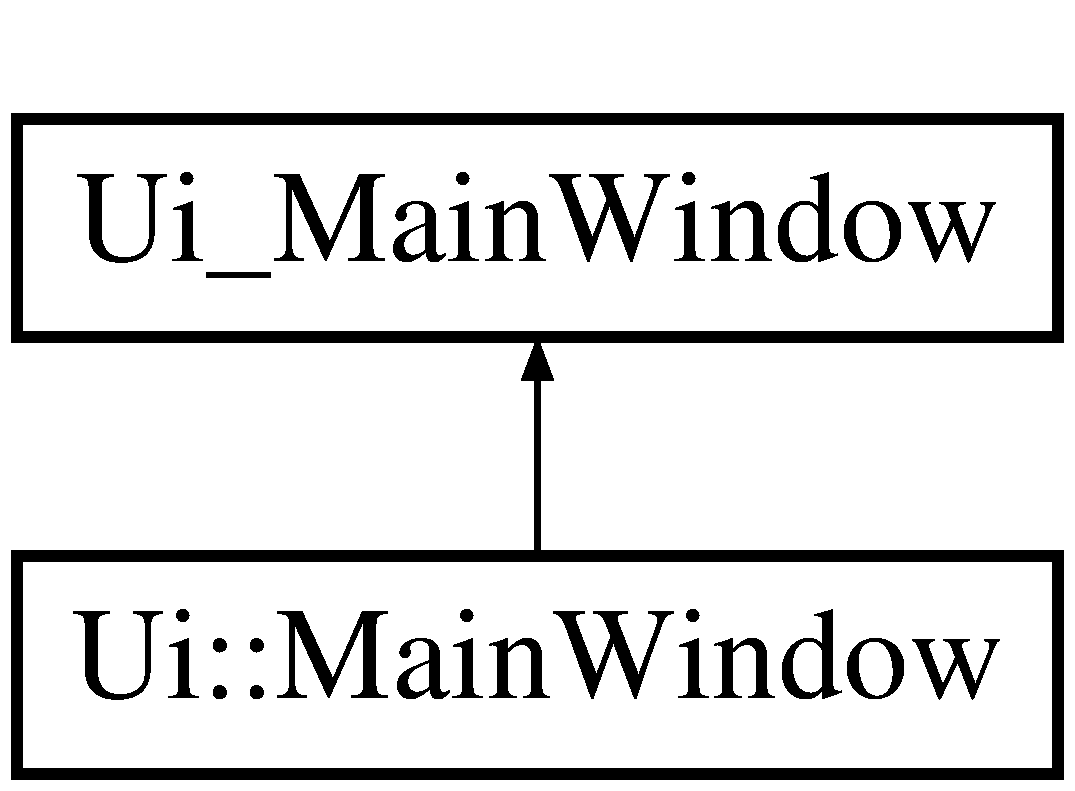
\includegraphics[height=2.000000cm]{class_ui___main_window}
\end{center}
\end{figure}
\subsection*{Membros Públicos}
\begin{DoxyCompactItemize}
\item 
void \mbox{\hyperlink{class_ui___main_window_acf4a0872c4c77d8f43a2ec66ed849b58}{setup\+Ui}} (Q\+Main\+Window $\ast$\mbox{\hyperlink{class_main_window}{Main\+Window}})
\item 
void \mbox{\hyperlink{class_ui___main_window_a097dd160c3534a204904cb374412c618}{retranslate\+Ui}} (Q\+Main\+Window $\ast$\mbox{\hyperlink{class_main_window}{Main\+Window}})
\end{DoxyCompactItemize}
\subsection*{Atributos Públicos}
\begin{DoxyCompactItemize}
\item 
Q\+Widget $\ast$ \mbox{\hyperlink{class_ui___main_window_a30075506c2116c3ed4ff25e07ae75f81}{central\+Widget}}
\item 
Q\+H\+Box\+Layout $\ast$ \mbox{\hyperlink{class_ui___main_window_a03ce63974cc69b067c91bbf285cceca8}{horizontal\+Layout\+\_\+3}}
\item 
Q\+Group\+Box $\ast$ \mbox{\hyperlink{class_ui___main_window_aef7cb3be8cecfc9aaf98f036a98781ce}{group\+Box}}
\item 
Q\+H\+Box\+Layout $\ast$ \mbox{\hyperlink{class_ui___main_window_acd6fdc9ebacc4b25b834162380d75ce8}{horizontal\+Layout}}
\item 
Q\+List\+Widget $\ast$ \mbox{\hyperlink{class_ui___main_window_ae647a15635ba8a0e5d5aec475db99d8f}{list\+Widget}}
\item 
Q\+Group\+Box $\ast$ \mbox{\hyperlink{class_ui___main_window_abb28acde35ffce4d0e6152579df2cbc3}{group\+Box\+\_\+2}}
\item 
Q\+H\+Box\+Layout $\ast$ \mbox{\hyperlink{class_ui___main_window_a80867018070156432923d0266cc9fe25}{horizontal\+Layout\+\_\+2}}
\item 
Q\+Text\+Browser $\ast$ \mbox{\hyperlink{class_ui___main_window_a2c789c07fa5fc1cee05aae8df52bb02d}{text\+Browser}}
\item 
Q\+Menu\+Bar $\ast$ \mbox{\hyperlink{class_ui___main_window_a2be1c24ec9adfca18e1dcc951931457f}{menu\+Bar}}
\item 
Q\+Tool\+Bar $\ast$ \mbox{\hyperlink{class_ui___main_window_a5172877001c8c7b4e0f6de50421867d1}{main\+Tool\+Bar}}
\item 
Q\+Status\+Bar $\ast$ \mbox{\hyperlink{class_ui___main_window_a50fa481337604bcc8bf68de18ab16ecd}{status\+Bar}}
\end{DoxyCompactItemize}


\subsection{Funções membros}
\mbox{\Hypertarget{class_ui___main_window_a097dd160c3534a204904cb374412c618}\label{class_ui___main_window_a097dd160c3534a204904cb374412c618}} 
\index{Ui\+\_\+\+Main\+Window@{Ui\+\_\+\+Main\+Window}!retranslate\+Ui@{retranslate\+Ui}}
\index{retranslate\+Ui@{retranslate\+Ui}!Ui\+\_\+\+Main\+Window@{Ui\+\_\+\+Main\+Window}}
\subsubsection{\texorpdfstring{retranslate\+Ui()}{retranslateUi()}}
{\footnotesize\ttfamily void Ui\+\_\+\+Main\+Window\+::retranslate\+Ui (\begin{DoxyParamCaption}\item[{Q\+Main\+Window $\ast$}]{Main\+Window }\end{DoxyParamCaption})\hspace{0.3cm}{\ttfamily [inline]}}


\begin{DoxyCode}
103     \{
104         \mbox{\hyperlink{class_main_window}{MainWindow}}->setWindowTitle(QApplication::translate(\textcolor{stringliteral}{"MainWindow"}, \textcolor{stringliteral}{"MainWindow"}, Q\_NULLPTR)
      );
105         \mbox{\hyperlink{class_ui___main_window_aef7cb3be8cecfc9aaf98f036a98781ce}{groupBox}}->setTitle(QApplication::translate(\textcolor{stringliteral}{"MainWindow"}, \textcolor{stringliteral}{"IPs do servidor"}, Q\_NULLPTR));
106         \mbox{\hyperlink{class_ui___main_window_abb28acde35ffce4d0e6152579df2cbc3}{groupBox\_2}}->setTitle(QApplication::translate(\textcolor{stringliteral}{"MainWindow"}, \textcolor{stringliteral}{"Mensagens"}, Q\_NULLPTR));
107     \} \textcolor{comment}{// retranslateUi}
\end{DoxyCode}
\mbox{\Hypertarget{class_ui___main_window_acf4a0872c4c77d8f43a2ec66ed849b58}\label{class_ui___main_window_acf4a0872c4c77d8f43a2ec66ed849b58}} 
\index{Ui\+\_\+\+Main\+Window@{Ui\+\_\+\+Main\+Window}!setup\+Ui@{setup\+Ui}}
\index{setup\+Ui@{setup\+Ui}!Ui\+\_\+\+Main\+Window@{Ui\+\_\+\+Main\+Window}}
\subsubsection{\texorpdfstring{setup\+Ui()}{setupUi()}}
{\footnotesize\ttfamily void Ui\+\_\+\+Main\+Window\+::setup\+Ui (\begin{DoxyParamCaption}\item[{Q\+Main\+Window $\ast$}]{Main\+Window }\end{DoxyParamCaption})\hspace{0.3cm}{\ttfamily [inline]}}


\begin{DoxyCode}
45     \{
46         \textcolor{keywordflow}{if} (\mbox{\hyperlink{class_main_window}{MainWindow}}->objectName().isEmpty())
47             \mbox{\hyperlink{class_main_window}{MainWindow}}->setObjectName(QStringLiteral(\textcolor{stringliteral}{"MainWindow"}));
48         \mbox{\hyperlink{class_main_window}{MainWindow}}->resize(634, 411);
49         \mbox{\hyperlink{class_ui___main_window_a30075506c2116c3ed4ff25e07ae75f81}{centralWidget}} = \textcolor{keyword}{new} QWidget(\mbox{\hyperlink{class_main_window}{MainWindow}});
50         \mbox{\hyperlink{class_ui___main_window_a30075506c2116c3ed4ff25e07ae75f81}{centralWidget}}->setObjectName(QStringLiteral(\textcolor{stringliteral}{"centralWidget"}));
51         \mbox{\hyperlink{class_ui___main_window_a03ce63974cc69b067c91bbf285cceca8}{horizontalLayout\_3}} = \textcolor{keyword}{new} QHBoxLayout(\mbox{\hyperlink{class_ui___main_window_a30075506c2116c3ed4ff25e07ae75f81}{centralWidget}});
52         \mbox{\hyperlink{class_ui___main_window_a03ce63974cc69b067c91bbf285cceca8}{horizontalLayout\_3}}->setSpacing(6);
53         \mbox{\hyperlink{class_ui___main_window_a03ce63974cc69b067c91bbf285cceca8}{horizontalLayout\_3}}->setContentsMargins(11, 11, 11, 11);
54         \mbox{\hyperlink{class_ui___main_window_a03ce63974cc69b067c91bbf285cceca8}{horizontalLayout\_3}}->setObjectName(QStringLiteral(\textcolor{stringliteral}{"horizontalLayout\_3"}));
55         \mbox{\hyperlink{class_ui___main_window_aef7cb3be8cecfc9aaf98f036a98781ce}{groupBox}} = \textcolor{keyword}{new} QGroupBox(\mbox{\hyperlink{class_ui___main_window_a30075506c2116c3ed4ff25e07ae75f81}{centralWidget}});
56         \mbox{\hyperlink{class_ui___main_window_aef7cb3be8cecfc9aaf98f036a98781ce}{groupBox}}->setObjectName(QStringLiteral(\textcolor{stringliteral}{"groupBox"}));
57         \mbox{\hyperlink{class_ui___main_window_acd6fdc9ebacc4b25b834162380d75ce8}{horizontalLayout}} = \textcolor{keyword}{new} QHBoxLayout(\mbox{\hyperlink{class_ui___main_window_aef7cb3be8cecfc9aaf98f036a98781ce}{groupBox}});
58         \mbox{\hyperlink{class_ui___main_window_acd6fdc9ebacc4b25b834162380d75ce8}{horizontalLayout}}->setSpacing(6);
59         \mbox{\hyperlink{class_ui___main_window_acd6fdc9ebacc4b25b834162380d75ce8}{horizontalLayout}}->setContentsMargins(11, 11, 11, 11);
60         \mbox{\hyperlink{class_ui___main_window_acd6fdc9ebacc4b25b834162380d75ce8}{horizontalLayout}}->setObjectName(QStringLiteral(\textcolor{stringliteral}{"horizontalLayout"}));
61         \mbox{\hyperlink{class_ui___main_window_ae647a15635ba8a0e5d5aec475db99d8f}{listWidget}} = \textcolor{keyword}{new} QListWidget(\mbox{\hyperlink{class_ui___main_window_aef7cb3be8cecfc9aaf98f036a98781ce}{groupBox}});
62         \mbox{\hyperlink{class_ui___main_window_ae647a15635ba8a0e5d5aec475db99d8f}{listWidget}}->setObjectName(QStringLiteral(\textcolor{stringliteral}{"listWidget"}));
63 
64         \mbox{\hyperlink{class_ui___main_window_acd6fdc9ebacc4b25b834162380d75ce8}{horizontalLayout}}->addWidget(\mbox{\hyperlink{class_ui___main_window_ae647a15635ba8a0e5d5aec475db99d8f}{listWidget}});
65 
66 
67         \mbox{\hyperlink{class_ui___main_window_a03ce63974cc69b067c91bbf285cceca8}{horizontalLayout\_3}}->addWidget(\mbox{\hyperlink{class_ui___main_window_aef7cb3be8cecfc9aaf98f036a98781ce}{groupBox}});
68 
69         \mbox{\hyperlink{class_ui___main_window_abb28acde35ffce4d0e6152579df2cbc3}{groupBox\_2}} = \textcolor{keyword}{new} QGroupBox(\mbox{\hyperlink{class_ui___main_window_a30075506c2116c3ed4ff25e07ae75f81}{centralWidget}});
70         \mbox{\hyperlink{class_ui___main_window_abb28acde35ffce4d0e6152579df2cbc3}{groupBox\_2}}->setObjectName(QStringLiteral(\textcolor{stringliteral}{"groupBox\_2"}));
71         \mbox{\hyperlink{class_ui___main_window_a80867018070156432923d0266cc9fe25}{horizontalLayout\_2}} = \textcolor{keyword}{new} QHBoxLayout(\mbox{\hyperlink{class_ui___main_window_abb28acde35ffce4d0e6152579df2cbc3}{groupBox\_2}});
72         \mbox{\hyperlink{class_ui___main_window_a80867018070156432923d0266cc9fe25}{horizontalLayout\_2}}->setSpacing(6);
73         \mbox{\hyperlink{class_ui___main_window_a80867018070156432923d0266cc9fe25}{horizontalLayout\_2}}->setContentsMargins(11, 11, 11, 11);
74         \mbox{\hyperlink{class_ui___main_window_a80867018070156432923d0266cc9fe25}{horizontalLayout\_2}}->setObjectName(QStringLiteral(\textcolor{stringliteral}{"horizontalLayout\_2"}));
75         \mbox{\hyperlink{class_ui___main_window_a2c789c07fa5fc1cee05aae8df52bb02d}{textBrowser}} = \textcolor{keyword}{new} QTextBrowser(\mbox{\hyperlink{class_ui___main_window_abb28acde35ffce4d0e6152579df2cbc3}{groupBox\_2}});
76         \mbox{\hyperlink{class_ui___main_window_a2c789c07fa5fc1cee05aae8df52bb02d}{textBrowser}}->setObjectName(QStringLiteral(\textcolor{stringliteral}{"textBrowser"}));
77 
78         \mbox{\hyperlink{class_ui___main_window_a80867018070156432923d0266cc9fe25}{horizontalLayout\_2}}->addWidget(\mbox{\hyperlink{class_ui___main_window_a2c789c07fa5fc1cee05aae8df52bb02d}{textBrowser}});
79 
80 
81         \mbox{\hyperlink{class_ui___main_window_a03ce63974cc69b067c91bbf285cceca8}{horizontalLayout\_3}}->addWidget(\mbox{\hyperlink{class_ui___main_window_abb28acde35ffce4d0e6152579df2cbc3}{groupBox\_2}});
82 
83         \mbox{\hyperlink{class_ui___main_window_a03ce63974cc69b067c91bbf285cceca8}{horizontalLayout\_3}}->setStretch(0, 40);
84         \mbox{\hyperlink{class_ui___main_window_a03ce63974cc69b067c91bbf285cceca8}{horizontalLayout\_3}}->setStretch(1, 60);
85         \mbox{\hyperlink{class_main_window}{MainWindow}}->setCentralWidget(\mbox{\hyperlink{class_ui___main_window_a30075506c2116c3ed4ff25e07ae75f81}{centralWidget}});
86         \mbox{\hyperlink{class_ui___main_window_a2be1c24ec9adfca18e1dcc951931457f}{menuBar}} = \textcolor{keyword}{new} QMenuBar(\mbox{\hyperlink{class_main_window}{MainWindow}});
87         \mbox{\hyperlink{class_ui___main_window_a2be1c24ec9adfca18e1dcc951931457f}{menuBar}}->setObjectName(QStringLiteral(\textcolor{stringliteral}{"menuBar"}));
88         \mbox{\hyperlink{class_ui___main_window_a2be1c24ec9adfca18e1dcc951931457f}{menuBar}}->setGeometry(QRect(0, 0, 634, 22));
89         \mbox{\hyperlink{class_main_window}{MainWindow}}->setMenuBar(\mbox{\hyperlink{class_ui___main_window_a2be1c24ec9adfca18e1dcc951931457f}{menuBar}});
90         \mbox{\hyperlink{class_ui___main_window_a5172877001c8c7b4e0f6de50421867d1}{mainToolBar}} = \textcolor{keyword}{new} QToolBar(\mbox{\hyperlink{class_main_window}{MainWindow}});
91         \mbox{\hyperlink{class_ui___main_window_a5172877001c8c7b4e0f6de50421867d1}{mainToolBar}}->setObjectName(QStringLiteral(\textcolor{stringliteral}{"mainToolBar"}));
92         \mbox{\hyperlink{class_main_window}{MainWindow}}->addToolBar(Qt::TopToolBarArea, \mbox{\hyperlink{class_ui___main_window_a5172877001c8c7b4e0f6de50421867d1}{mainToolBar}});
93         \mbox{\hyperlink{class_ui___main_window_a50fa481337604bcc8bf68de18ab16ecd}{statusBar}} = \textcolor{keyword}{new} QStatusBar(\mbox{\hyperlink{class_main_window}{MainWindow}});
94         \mbox{\hyperlink{class_ui___main_window_a50fa481337604bcc8bf68de18ab16ecd}{statusBar}}->setObjectName(QStringLiteral(\textcolor{stringliteral}{"statusBar"}));
95         \mbox{\hyperlink{class_main_window}{MainWindow}}->setStatusBar(\mbox{\hyperlink{class_ui___main_window_a50fa481337604bcc8bf68de18ab16ecd}{statusBar}});
96 
97         \mbox{\hyperlink{class_ui___main_window_a097dd160c3534a204904cb374412c618}{retranslateUi}}(\mbox{\hyperlink{class_main_window}{MainWindow}});
98 
99         QMetaObject::connectSlotsByName(\mbox{\hyperlink{class_main_window}{MainWindow}});
100     \} \textcolor{comment}{// setupUi}
\end{DoxyCode}


\subsection{Atributos}
\mbox{\Hypertarget{class_ui___main_window_a30075506c2116c3ed4ff25e07ae75f81}\label{class_ui___main_window_a30075506c2116c3ed4ff25e07ae75f81}} 
\index{Ui\+\_\+\+Main\+Window@{Ui\+\_\+\+Main\+Window}!central\+Widget@{central\+Widget}}
\index{central\+Widget@{central\+Widget}!Ui\+\_\+\+Main\+Window@{Ui\+\_\+\+Main\+Window}}
\subsubsection{\texorpdfstring{central\+Widget}{centralWidget}}
{\footnotesize\ttfamily Q\+Widget$\ast$ Ui\+\_\+\+Main\+Window\+::central\+Widget}

\mbox{\Hypertarget{class_ui___main_window_aef7cb3be8cecfc9aaf98f036a98781ce}\label{class_ui___main_window_aef7cb3be8cecfc9aaf98f036a98781ce}} 
\index{Ui\+\_\+\+Main\+Window@{Ui\+\_\+\+Main\+Window}!group\+Box@{group\+Box}}
\index{group\+Box@{group\+Box}!Ui\+\_\+\+Main\+Window@{Ui\+\_\+\+Main\+Window}}
\subsubsection{\texorpdfstring{group\+Box}{groupBox}}
{\footnotesize\ttfamily Q\+Group\+Box$\ast$ Ui\+\_\+\+Main\+Window\+::group\+Box}

\mbox{\Hypertarget{class_ui___main_window_abb28acde35ffce4d0e6152579df2cbc3}\label{class_ui___main_window_abb28acde35ffce4d0e6152579df2cbc3}} 
\index{Ui\+\_\+\+Main\+Window@{Ui\+\_\+\+Main\+Window}!group\+Box\+\_\+2@{group\+Box\+\_\+2}}
\index{group\+Box\+\_\+2@{group\+Box\+\_\+2}!Ui\+\_\+\+Main\+Window@{Ui\+\_\+\+Main\+Window}}
\subsubsection{\texorpdfstring{group\+Box\+\_\+2}{groupBox\_2}}
{\footnotesize\ttfamily Q\+Group\+Box$\ast$ Ui\+\_\+\+Main\+Window\+::group\+Box\+\_\+2}

\mbox{\Hypertarget{class_ui___main_window_acd6fdc9ebacc4b25b834162380d75ce8}\label{class_ui___main_window_acd6fdc9ebacc4b25b834162380d75ce8}} 
\index{Ui\+\_\+\+Main\+Window@{Ui\+\_\+\+Main\+Window}!horizontal\+Layout@{horizontal\+Layout}}
\index{horizontal\+Layout@{horizontal\+Layout}!Ui\+\_\+\+Main\+Window@{Ui\+\_\+\+Main\+Window}}
\subsubsection{\texorpdfstring{horizontal\+Layout}{horizontalLayout}}
{\footnotesize\ttfamily Q\+H\+Box\+Layout$\ast$ Ui\+\_\+\+Main\+Window\+::horizontal\+Layout}

\mbox{\Hypertarget{class_ui___main_window_a80867018070156432923d0266cc9fe25}\label{class_ui___main_window_a80867018070156432923d0266cc9fe25}} 
\index{Ui\+\_\+\+Main\+Window@{Ui\+\_\+\+Main\+Window}!horizontal\+Layout\+\_\+2@{horizontal\+Layout\+\_\+2}}
\index{horizontal\+Layout\+\_\+2@{horizontal\+Layout\+\_\+2}!Ui\+\_\+\+Main\+Window@{Ui\+\_\+\+Main\+Window}}
\subsubsection{\texorpdfstring{horizontal\+Layout\+\_\+2}{horizontalLayout\_2}}
{\footnotesize\ttfamily Q\+H\+Box\+Layout$\ast$ Ui\+\_\+\+Main\+Window\+::horizontal\+Layout\+\_\+2}

\mbox{\Hypertarget{class_ui___main_window_a03ce63974cc69b067c91bbf285cceca8}\label{class_ui___main_window_a03ce63974cc69b067c91bbf285cceca8}} 
\index{Ui\+\_\+\+Main\+Window@{Ui\+\_\+\+Main\+Window}!horizontal\+Layout\+\_\+3@{horizontal\+Layout\+\_\+3}}
\index{horizontal\+Layout\+\_\+3@{horizontal\+Layout\+\_\+3}!Ui\+\_\+\+Main\+Window@{Ui\+\_\+\+Main\+Window}}
\subsubsection{\texorpdfstring{horizontal\+Layout\+\_\+3}{horizontalLayout\_3}}
{\footnotesize\ttfamily Q\+H\+Box\+Layout$\ast$ Ui\+\_\+\+Main\+Window\+::horizontal\+Layout\+\_\+3}

\mbox{\Hypertarget{class_ui___main_window_ae647a15635ba8a0e5d5aec475db99d8f}\label{class_ui___main_window_ae647a15635ba8a0e5d5aec475db99d8f}} 
\index{Ui\+\_\+\+Main\+Window@{Ui\+\_\+\+Main\+Window}!list\+Widget@{list\+Widget}}
\index{list\+Widget@{list\+Widget}!Ui\+\_\+\+Main\+Window@{Ui\+\_\+\+Main\+Window}}
\subsubsection{\texorpdfstring{list\+Widget}{listWidget}}
{\footnotesize\ttfamily Q\+List\+Widget$\ast$ Ui\+\_\+\+Main\+Window\+::list\+Widget}

\mbox{\Hypertarget{class_ui___main_window_a5172877001c8c7b4e0f6de50421867d1}\label{class_ui___main_window_a5172877001c8c7b4e0f6de50421867d1}} 
\index{Ui\+\_\+\+Main\+Window@{Ui\+\_\+\+Main\+Window}!main\+Tool\+Bar@{main\+Tool\+Bar}}
\index{main\+Tool\+Bar@{main\+Tool\+Bar}!Ui\+\_\+\+Main\+Window@{Ui\+\_\+\+Main\+Window}}
\subsubsection{\texorpdfstring{main\+Tool\+Bar}{mainToolBar}}
{\footnotesize\ttfamily Q\+Tool\+Bar$\ast$ Ui\+\_\+\+Main\+Window\+::main\+Tool\+Bar}

\mbox{\Hypertarget{class_ui___main_window_a2be1c24ec9adfca18e1dcc951931457f}\label{class_ui___main_window_a2be1c24ec9adfca18e1dcc951931457f}} 
\index{Ui\+\_\+\+Main\+Window@{Ui\+\_\+\+Main\+Window}!menu\+Bar@{menu\+Bar}}
\index{menu\+Bar@{menu\+Bar}!Ui\+\_\+\+Main\+Window@{Ui\+\_\+\+Main\+Window}}
\subsubsection{\texorpdfstring{menu\+Bar}{menuBar}}
{\footnotesize\ttfamily Q\+Menu\+Bar$\ast$ Ui\+\_\+\+Main\+Window\+::menu\+Bar}

\mbox{\Hypertarget{class_ui___main_window_a50fa481337604bcc8bf68de18ab16ecd}\label{class_ui___main_window_a50fa481337604bcc8bf68de18ab16ecd}} 
\index{Ui\+\_\+\+Main\+Window@{Ui\+\_\+\+Main\+Window}!status\+Bar@{status\+Bar}}
\index{status\+Bar@{status\+Bar}!Ui\+\_\+\+Main\+Window@{Ui\+\_\+\+Main\+Window}}
\subsubsection{\texorpdfstring{status\+Bar}{statusBar}}
{\footnotesize\ttfamily Q\+Status\+Bar$\ast$ Ui\+\_\+\+Main\+Window\+::status\+Bar}

\mbox{\Hypertarget{class_ui___main_window_a2c789c07fa5fc1cee05aae8df52bb02d}\label{class_ui___main_window_a2c789c07fa5fc1cee05aae8df52bb02d}} 
\index{Ui\+\_\+\+Main\+Window@{Ui\+\_\+\+Main\+Window}!text\+Browser@{text\+Browser}}
\index{text\+Browser@{text\+Browser}!Ui\+\_\+\+Main\+Window@{Ui\+\_\+\+Main\+Window}}
\subsubsection{\texorpdfstring{text\+Browser}{textBrowser}}
{\footnotesize\ttfamily Q\+Text\+Browser$\ast$ Ui\+\_\+\+Main\+Window\+::text\+Browser}



A documentação para essa classe foi gerada a partir do seguinte arquivo\+:\begin{DoxyCompactItemize}
\item 
C\+:/\+Users/mateu/\+Documents/\+Projeto Final D\+C\+A 1202/\+Qt\+Tcp\+Server/\mbox{\hyperlink{ui__mainwindow_8h}{ui\+\_\+mainwindow.\+h}}\end{DoxyCompactItemize}

\chapter{Arquivos}
\hypertarget{datastorage_8cpp}{}\section{Referência do Arquivo C\+:/\+Users/mateu/\+Documents/\+Projeto Final D\+CA 1202/\+Qt\+Tcp\+Server/datastorage.cpp}
\label{datastorage_8cpp}\index{C\+:/\+Users/mateu/\+Documents/\+Projeto Final D\+C\+A 1202/\+Qt\+Tcp\+Server/datastorage.\+cpp@{C\+:/\+Users/mateu/\+Documents/\+Projeto Final D\+C\+A 1202/\+Qt\+Tcp\+Server/datastorage.\+cpp}}
{\ttfamily \#include \char`\"{}datastorage.\+h\char`\"{}}\newline
{\ttfamily \#include $<$Q\+Mutex\+Locker$>$}\newline
{\ttfamily \#include $<$Q\+Debug$>$}\newline
\subsection*{Componentes}
\begin{DoxyCompactItemize}
\item 
struct \mbox{\hyperlink{struct_range_test}{Range\+Test}}
\end{DoxyCompactItemize}

\hypertarget{datastorage_8h}{}\section{Referência do Arquivo C\+:/\+Users/mateu/\+Documents/\+Projeto Final D\+CA 1202/\+Qt\+Tcp\+Server/datastorage.h}
\label{datastorage_8h}\index{C\+:/\+Users/mateu/\+Documents/\+Projeto Final D\+C\+A 1202/\+Qt\+Tcp\+Server/datastorage.\+h@{C\+:/\+Users/mateu/\+Documents/\+Projeto Final D\+C\+A 1202/\+Qt\+Tcp\+Server/datastorage.\+h}}
{\ttfamily \#include $<$Q\+Date\+Time$>$}\newline
{\ttfamily \#include $<$Q\+Host\+Address$>$}\newline
{\ttfamily \#include $<$Q\+Mutex$>$}\newline
{\ttfamily \#include $<$Q\+Map$>$}\newline
{\ttfamily \#include $<$vector$>$}\newline
\subsection*{Componentes}
\begin{DoxyCompactItemize}
\item 
struct \mbox{\hyperlink{struct_entry}{Entry}}
\item 
class \mbox{\hyperlink{class_data_storage}{Data\+Storage}}
\end{DoxyCompactItemize}

\hypertarget{main_8cpp}{}\section{Referência do Arquivo C\+:/\+Users/mateu/\+Documents/\+Projeto Final D\+CA 1202/\+Cliente\+\_\+\+Produtor/main.cpp}
\label{main_8cpp}\index{C\+:/\+Users/mateu/\+Documents/\+Projeto Final D\+C\+A 1202/\+Cliente\+\_\+\+Produtor/main.\+cpp@{C\+:/\+Users/mateu/\+Documents/\+Projeto Final D\+C\+A 1202/\+Cliente\+\_\+\+Produtor/main.\+cpp}}
{\ttfamily \#include \char`\"{}mainwindow.\+h\char`\"{}}\newline
{\ttfamily \#include $<$Q\+Application$>$}\newline
\subsection*{Funções}
\begin{DoxyCompactItemize}
\item 
int \mbox{\hyperlink{main_8cpp_a0ddf1224851353fc92bfbff6f499fa97}{main}} (int argc, char $\ast$argv\mbox{[}$\,$\mbox{]})
\end{DoxyCompactItemize}


\subsection{Funções}
\mbox{\Hypertarget{main_8cpp_a0ddf1224851353fc92bfbff6f499fa97}\label{main_8cpp_a0ddf1224851353fc92bfbff6f499fa97}} 
\index{main.\+cpp@{main.\+cpp}!main@{main}}
\index{main@{main}!main.\+cpp@{main.\+cpp}}
\subsubsection{\texorpdfstring{main()}{main()}}
{\footnotesize\ttfamily int main (\begin{DoxyParamCaption}\item[{int}]{argc,  }\item[{char $\ast$}]{argv\mbox{[}$\,$\mbox{]} }\end{DoxyParamCaption})}


\begin{DoxyCode}
5 \{
6   QApplication a(argc, argv);
7   \mbox{\hyperlink{class_main_window}{MainWindow}} w;
8   w.show();
9 
10   \textcolor{keywordflow}{return} a.exec();
11 \}
\end{DoxyCode}

\hypertarget{mainwindow_8cpp}{}\section{Referência do Arquivo C\+:/\+Users/mateu/\+Documents/\+Projeto Final D\+CA 1202/\+Qt\+Tcp\+Server/mainwindow.cpp}
\label{mainwindow_8cpp}\index{C\+:/\+Users/mateu/\+Documents/\+Projeto Final D\+C\+A 1202/\+Qt\+Tcp\+Server/mainwindow.\+cpp@{C\+:/\+Users/mateu/\+Documents/\+Projeto Final D\+C\+A 1202/\+Qt\+Tcp\+Server/mainwindow.\+cpp}}
{\ttfamily \#include \char`\"{}mainwindow.\+h\char`\"{}}\newline
{\ttfamily \#include \char`\"{}ui\+\_\+mainwindow.\+h\char`\"{}}\newline
{\ttfamily \#include \char`\"{}myserver.\+h\char`\"{}}\newline
{\ttfamily \#include $<$Q\+String\+List$>$}\newline

\hypertarget{mainwindow_8h}{}\section{Referência do Arquivo C\+:/\+Users/mateu/\+Documents/\+Projeto Final D\+CA 1202/\+Cliente\+\_\+\+Produtor/mainwindow.h}
\label{mainwindow_8h}\index{C\+:/\+Users/mateu/\+Documents/\+Projeto Final D\+C\+A 1202/\+Cliente\+\_\+\+Produtor/mainwindow.\+h@{C\+:/\+Users/mateu/\+Documents/\+Projeto Final D\+C\+A 1202/\+Cliente\+\_\+\+Produtor/mainwindow.\+h}}
{\ttfamily \#include $<$Q\+Main\+Window$>$}\newline
{\ttfamily \#include $<$Q\+Tcp\+Socket$>$}\newline
{\ttfamily \#include $<$Q\+Debug$>$}\newline
{\ttfamily \#include $<$Q\+Timer$>$}\newline
\subsection*{Componentes}
\begin{DoxyCompactItemize}
\item 
class \mbox{\hyperlink{class_main_window}{Main\+Window}}
\end{DoxyCompactItemize}
\subsection*{$<$em$>$Namespaces$<$/em$>$}
\begin{DoxyCompactItemize}
\item 
 \mbox{\hyperlink{namespace_ui}{Ui}}
\end{DoxyCompactItemize}

\hypertarget{moc__mainwindow_8cpp}{}\section{Referência do Arquivo C\+:/\+Users/mateu/\+Documents/\+Projeto Final D\+CA 1202/\+Qt\+Tcp\+Server/moc\+\_\+mainwindow.cpp}
\label{moc__mainwindow_8cpp}\index{C\+:/\+Users/mateu/\+Documents/\+Projeto Final D\+C\+A 1202/\+Qt\+Tcp\+Server/moc\+\_\+mainwindow.\+cpp@{C\+:/\+Users/mateu/\+Documents/\+Projeto Final D\+C\+A 1202/\+Qt\+Tcp\+Server/moc\+\_\+mainwindow.\+cpp}}
{\ttfamily \#include \char`\"{}mainwindow.\+h\char`\"{}}\newline
{\ttfamily \#include $<$Qt\+Core/qbytearray.\+h$>$}\newline
{\ttfamily \#include $<$Qt\+Core/qmetatype.\+h$>$}\newline
\subsection*{Componentes}
\begin{DoxyCompactItemize}
\item 
struct \mbox{\hyperlink{structqt__meta__stringdata___main_window__t}{qt\+\_\+meta\+\_\+stringdata\+\_\+\+Main\+Window\+\_\+t}}
\end{DoxyCompactItemize}
\subsection*{Definições e Macros}
\begin{DoxyCompactItemize}
\item 
\#define \mbox{\hyperlink{moc__mainwindow_8cpp_a75bb9482d242cde0a06c9dbdc6b83abe}{Q\+T\+\_\+\+M\+O\+C\+\_\+\+L\+I\+T\+E\+R\+AL}}(idx,  ofs,  len)
\end{DoxyCompactItemize}


\subsection{Definições e macros}
\mbox{\Hypertarget{moc__mainwindow_8cpp_a75bb9482d242cde0a06c9dbdc6b83abe}\label{moc__mainwindow_8cpp_a75bb9482d242cde0a06c9dbdc6b83abe}} 
\index{moc\+\_\+mainwindow.\+cpp@{moc\+\_\+mainwindow.\+cpp}!Q\+T\+\_\+\+M\+O\+C\+\_\+\+L\+I\+T\+E\+R\+AL@{Q\+T\+\_\+\+M\+O\+C\+\_\+\+L\+I\+T\+E\+R\+AL}}
\index{Q\+T\+\_\+\+M\+O\+C\+\_\+\+L\+I\+T\+E\+R\+AL@{Q\+T\+\_\+\+M\+O\+C\+\_\+\+L\+I\+T\+E\+R\+AL}!moc\+\_\+mainwindow.\+cpp@{moc\+\_\+mainwindow.\+cpp}}
\subsubsection{\texorpdfstring{Q\+T\+\_\+\+M\+O\+C\+\_\+\+L\+I\+T\+E\+R\+AL}{QT\_MOC\_LITERAL}}
{\footnotesize\ttfamily \#define Q\+T\+\_\+\+M\+O\+C\+\_\+\+L\+I\+T\+E\+R\+AL(\begin{DoxyParamCaption}\item[{}]{idx,  }\item[{}]{ofs,  }\item[{}]{len }\end{DoxyParamCaption})}

{\bfseries Valor\+:}
\begin{DoxyCode}
Q\_STATIC\_BYTE\_ARRAY\_DATA\_HEADER\_INITIALIZER\_WITH\_OFFSET(len, \(\backslash\)
    qptrdiff(offsetof(\mbox{\hyperlink{structqt__meta__stringdata___main_window__t}{qt\_meta\_stringdata\_MainWindow\_t}}, stringdata0) + ofs \(\backslash\)
        - idx * \textcolor{keyword}{sizeof}(QByteArrayData)) \(\backslash\)
    )
\end{DoxyCode}

\hypertarget{moc__myserver_8cpp}{}\section{Referência do Arquivo C\+:/\+Users/mateu/\+Documents/\+Projeto Final D\+CA 1202/\+Qt\+Tcp\+Server/moc\+\_\+myserver.cpp}
\label{moc__myserver_8cpp}\index{C\+:/\+Users/mateu/\+Documents/\+Projeto Final D\+C\+A 1202/\+Qt\+Tcp\+Server/moc\+\_\+myserver.\+cpp@{C\+:/\+Users/mateu/\+Documents/\+Projeto Final D\+C\+A 1202/\+Qt\+Tcp\+Server/moc\+\_\+myserver.\+cpp}}
{\ttfamily \#include \char`\"{}myserver.\+h\char`\"{}}\newline
{\ttfamily \#include $<$Qt\+Core/qbytearray.\+h$>$}\newline
{\ttfamily \#include $<$Qt\+Core/qmetatype.\+h$>$}\newline
\subsection*{Componentes}
\begin{DoxyCompactItemize}
\item 
struct \mbox{\hyperlink{structqt__meta__stringdata___my_server__t}{qt\+\_\+meta\+\_\+stringdata\+\_\+\+My\+Server\+\_\+t}}
\end{DoxyCompactItemize}
\subsection*{Definições e Macros}
\begin{DoxyCompactItemize}
\item 
\#define \mbox{\hyperlink{moc__myserver_8cpp_a75bb9482d242cde0a06c9dbdc6b83abe}{Q\+T\+\_\+\+M\+O\+C\+\_\+\+L\+I\+T\+E\+R\+AL}}(idx,  ofs,  len)
\end{DoxyCompactItemize}


\subsection{Definições e macros}
\mbox{\Hypertarget{moc__myserver_8cpp_a75bb9482d242cde0a06c9dbdc6b83abe}\label{moc__myserver_8cpp_a75bb9482d242cde0a06c9dbdc6b83abe}} 
\index{moc\+\_\+myserver.\+cpp@{moc\+\_\+myserver.\+cpp}!Q\+T\+\_\+\+M\+O\+C\+\_\+\+L\+I\+T\+E\+R\+AL@{Q\+T\+\_\+\+M\+O\+C\+\_\+\+L\+I\+T\+E\+R\+AL}}
\index{Q\+T\+\_\+\+M\+O\+C\+\_\+\+L\+I\+T\+E\+R\+AL@{Q\+T\+\_\+\+M\+O\+C\+\_\+\+L\+I\+T\+E\+R\+AL}!moc\+\_\+myserver.\+cpp@{moc\+\_\+myserver.\+cpp}}
\subsubsection{\texorpdfstring{Q\+T\+\_\+\+M\+O\+C\+\_\+\+L\+I\+T\+E\+R\+AL}{QT\_MOC\_LITERAL}}
{\footnotesize\ttfamily \#define Q\+T\+\_\+\+M\+O\+C\+\_\+\+L\+I\+T\+E\+R\+AL(\begin{DoxyParamCaption}\item[{}]{idx,  }\item[{}]{ofs,  }\item[{}]{len }\end{DoxyParamCaption})}

{\bfseries Valor\+:}
\begin{DoxyCode}
Q\_STATIC\_BYTE\_ARRAY\_DATA\_HEADER\_INITIALIZER\_WITH\_OFFSET(len, \(\backslash\)
    qptrdiff(offsetof(\mbox{\hyperlink{structqt__meta__stringdata___my_server__t}{qt\_meta\_stringdata\_MyServer\_t}}, stringdata0) + ofs \(\backslash\)
        - idx * \textcolor{keyword}{sizeof}(QByteArrayData)) \(\backslash\)
    )
\end{DoxyCode}

\hypertarget{moc__mythread_8cpp}{}\section{Referência do Arquivo C\+:/\+Users/mateu/\+Documents/\+Projeto Final D\+CA 1202/\+Qt\+Tcp\+Server/moc\+\_\+mythread.cpp}
\label{moc__mythread_8cpp}\index{C\+:/\+Users/mateu/\+Documents/\+Projeto Final D\+C\+A 1202/\+Qt\+Tcp\+Server/moc\+\_\+mythread.\+cpp@{C\+:/\+Users/mateu/\+Documents/\+Projeto Final D\+C\+A 1202/\+Qt\+Tcp\+Server/moc\+\_\+mythread.\+cpp}}
{\ttfamily \#include \char`\"{}mythread.\+h\char`\"{}}\newline
{\ttfamily \#include $<$Qt\+Core/qbytearray.\+h$>$}\newline
{\ttfamily \#include $<$Qt\+Core/qmetatype.\+h$>$}\newline
\subsection*{Componentes}
\begin{DoxyCompactItemize}
\item 
struct \mbox{\hyperlink{structqt__meta__stringdata___my_thread__t}{qt\+\_\+meta\+\_\+stringdata\+\_\+\+My\+Thread\+\_\+t}}
\end{DoxyCompactItemize}
\subsection*{Definições e Macros}
\begin{DoxyCompactItemize}
\item 
\#define \mbox{\hyperlink{moc__mythread_8cpp_a75bb9482d242cde0a06c9dbdc6b83abe}{Q\+T\+\_\+\+M\+O\+C\+\_\+\+L\+I\+T\+E\+R\+AL}}(idx,  ofs,  len)
\end{DoxyCompactItemize}


\subsection{Definições e macros}
\mbox{\Hypertarget{moc__mythread_8cpp_a75bb9482d242cde0a06c9dbdc6b83abe}\label{moc__mythread_8cpp_a75bb9482d242cde0a06c9dbdc6b83abe}} 
\index{moc\+\_\+mythread.\+cpp@{moc\+\_\+mythread.\+cpp}!Q\+T\+\_\+\+M\+O\+C\+\_\+\+L\+I\+T\+E\+R\+AL@{Q\+T\+\_\+\+M\+O\+C\+\_\+\+L\+I\+T\+E\+R\+AL}}
\index{Q\+T\+\_\+\+M\+O\+C\+\_\+\+L\+I\+T\+E\+R\+AL@{Q\+T\+\_\+\+M\+O\+C\+\_\+\+L\+I\+T\+E\+R\+AL}!moc\+\_\+mythread.\+cpp@{moc\+\_\+mythread.\+cpp}}
\subsubsection{\texorpdfstring{Q\+T\+\_\+\+M\+O\+C\+\_\+\+L\+I\+T\+E\+R\+AL}{QT\_MOC\_LITERAL}}
{\footnotesize\ttfamily \#define Q\+T\+\_\+\+M\+O\+C\+\_\+\+L\+I\+T\+E\+R\+AL(\begin{DoxyParamCaption}\item[{}]{idx,  }\item[{}]{ofs,  }\item[{}]{len }\end{DoxyParamCaption})}

{\bfseries Valor\+:}
\begin{DoxyCode}
Q\_STATIC\_BYTE\_ARRAY\_DATA\_HEADER\_INITIALIZER\_WITH\_OFFSET(len, \(\backslash\)
    qptrdiff(offsetof(\mbox{\hyperlink{structqt__meta__stringdata___my_thread__t}{qt\_meta\_stringdata\_MyThread\_t}}, stringdata0) + ofs \(\backslash\)
        - idx * \textcolor{keyword}{sizeof}(QByteArrayData)) \(\backslash\)
    )
\end{DoxyCode}

\hypertarget{myserver_8cpp}{}\section{Referência do Arquivo C\+:/\+Users/mateu/\+Documents/\+Projeto Final D\+CA 1202/\+Qt\+Tcp\+Server/myserver.cpp}
\label{myserver_8cpp}\index{C\+:/\+Users/mateu/\+Documents/\+Projeto Final D\+C\+A 1202/\+Qt\+Tcp\+Server/myserver.\+cpp@{C\+:/\+Users/mateu/\+Documents/\+Projeto Final D\+C\+A 1202/\+Qt\+Tcp\+Server/myserver.\+cpp}}
{\ttfamily \#include \char`\"{}myserver.\+h\char`\"{}}\newline
{\ttfamily \#include $<$Q\+Network\+Interface$>$}\newline

\hypertarget{myserver_8h}{}\section{Referência do Arquivo C\+:/\+Users/mateu/\+Documents/\+Projeto Final D\+CA 1202/\+Qt\+Tcp\+Server/myserver.h}
\label{myserver_8h}\index{C\+:/\+Users/mateu/\+Documents/\+Projeto Final D\+C\+A 1202/\+Qt\+Tcp\+Server/myserver.\+h@{C\+:/\+Users/mateu/\+Documents/\+Projeto Final D\+C\+A 1202/\+Qt\+Tcp\+Server/myserver.\+h}}
{\ttfamily \#include $<$Q\+Tcp\+Server$>$}\newline
{\ttfamily \#include $<$Q\+Debug$>$}\newline
{\ttfamily \#include $<$Q\+String\+List$>$}\newline
{\ttfamily \#include \char`\"{}mythread.\+h\char`\"{}}\newline
{\ttfamily \#include \char`\"{}datastorage.\+h\char`\"{}}\newline
\subsection*{Componentes}
\begin{DoxyCompactItemize}
\item 
class \mbox{\hyperlink{class_my_server}{My\+Server}}
\begin{DoxyCompactList}\small\item\em The \mbox{\hyperlink{class_my_server}{My\+Server}} class inicia um servidor T\+CP capaz de \char`\"{}ouvir\char`\"{} a porta 1234. \end{DoxyCompactList}\end{DoxyCompactItemize}

\hypertarget{mythread_8cpp}{}\section{Referência do Arquivo C\+:/\+Users/mateu/\+Documents/\+Projeto Final D\+CA 1202/\+Qt\+Tcp\+Server/mythread.cpp}
\label{mythread_8cpp}\index{C\+:/\+Users/mateu/\+Documents/\+Projeto Final D\+C\+A 1202/\+Qt\+Tcp\+Server/mythread.\+cpp@{C\+:/\+Users/mateu/\+Documents/\+Projeto Final D\+C\+A 1202/\+Qt\+Tcp\+Server/mythread.\+cpp}}
{\ttfamily \#include \char`\"{}mythread.\+h\char`\"{}}\newline
{\ttfamily \#include $<$vector$>$}\newline

\hypertarget{mythread_8h}{}\section{Referência do Arquivo C\+:/\+Users/mateu/\+Documents/\+Projeto Final D\+CA 1202/\+Qt\+Tcp\+Server/mythread.h}
\label{mythread_8h}\index{C\+:/\+Users/mateu/\+Documents/\+Projeto Final D\+C\+A 1202/\+Qt\+Tcp\+Server/mythread.\+h@{C\+:/\+Users/mateu/\+Documents/\+Projeto Final D\+C\+A 1202/\+Qt\+Tcp\+Server/mythread.\+h}}
{\ttfamily \#include $<$Q\+Object$>$}\newline
{\ttfamily \#include $<$Q\+Thread$>$}\newline
{\ttfamily \#include $<$Q\+Tcp\+Socket$>$}\newline
{\ttfamily \#include $<$Q\+Debug$>$}\newline
{\ttfamily \#include $<$Q\+String\+List$>$}\newline
{\ttfamily \#include $<$Q\+String$>$}\newline
{\ttfamily \#include $<$Q\+Host\+Address$>$}\newline
{\ttfamily \#include \char`\"{}datastorage.\+h\char`\"{}}\newline
\subsection*{Componentes}
\begin{DoxyCompactItemize}
\item 
class \mbox{\hyperlink{class_my_thread}{My\+Thread}}
\begin{DoxyCompactList}\small\item\em The \mbox{\hyperlink{class_my_thread}{My\+Thread}} class cria uma thread que lida com o tratamento de uma conexao T\+CP de entrada. \end{DoxyCompactList}\end{DoxyCompactItemize}

\hypertarget{ui__mainwindow_8h}{}\section{Referência do Arquivo C\+:/\+Users/mateu/\+Documents/\+Projeto Final D\+CA 1202/\+Qt\+Tcp\+Server/ui\+\_\+mainwindow.h}
\label{ui__mainwindow_8h}\index{C\+:/\+Users/mateu/\+Documents/\+Projeto Final D\+C\+A 1202/\+Qt\+Tcp\+Server/ui\+\_\+mainwindow.\+h@{C\+:/\+Users/mateu/\+Documents/\+Projeto Final D\+C\+A 1202/\+Qt\+Tcp\+Server/ui\+\_\+mainwindow.\+h}}
{\ttfamily \#include $<$Qt\+Core/\+Q\+Variant$>$}\newline
{\ttfamily \#include $<$Qt\+Widgets/\+Q\+Action$>$}\newline
{\ttfamily \#include $<$Qt\+Widgets/\+Q\+Application$>$}\newline
{\ttfamily \#include $<$Qt\+Widgets/\+Q\+Button\+Group$>$}\newline
{\ttfamily \#include $<$Qt\+Widgets/\+Q\+Group\+Box$>$}\newline
{\ttfamily \#include $<$Qt\+Widgets/\+Q\+H\+Box\+Layout$>$}\newline
{\ttfamily \#include $<$Qt\+Widgets/\+Q\+Header\+View$>$}\newline
{\ttfamily \#include $<$Qt\+Widgets/\+Q\+List\+Widget$>$}\newline
{\ttfamily \#include $<$Qt\+Widgets/\+Q\+Main\+Window$>$}\newline
{\ttfamily \#include $<$Qt\+Widgets/\+Q\+Menu\+Bar$>$}\newline
{\ttfamily \#include $<$Qt\+Widgets/\+Q\+Status\+Bar$>$}\newline
{\ttfamily \#include $<$Qt\+Widgets/\+Q\+Text\+Browser$>$}\newline
{\ttfamily \#include $<$Qt\+Widgets/\+Q\+Tool\+Bar$>$}\newline
{\ttfamily \#include $<$Qt\+Widgets/\+Q\+Widget$>$}\newline
\subsection*{Componentes}
\begin{DoxyCompactItemize}
\item 
class \mbox{\hyperlink{class_ui___main_window}{Ui\+\_\+\+Main\+Window}}
\item 
class \mbox{\hyperlink{class_ui_1_1_main_window}{Ui\+::\+Main\+Window}}
\end{DoxyCompactItemize}
\subsection*{$<$em$>$Namespaces$<$/em$>$}
\begin{DoxyCompactItemize}
\item 
 \mbox{\hyperlink{namespace_ui}{Ui}}
\end{DoxyCompactItemize}

%--- End generated contents ---

% Index
\backmatter
\newpage
\phantomsection
\clearemptydoublepage
\addcontentsline{toc}{chapter}{Sumário}
\printindex

\end{document}
